% uklad dokumentu
	\documentclass{article}
	\usepackage{xparse}
	\usepackage[margin=1.5cm]{geometry}
    \usepackage{enumerate} 
	\frenchspacing
    \linespread{1.0}
    \setlength{\parindent}{0pt}

% jezyk polski
	\usepackage[T1]{fontenc}
	\usepackage[polish]{babel}
	\usepackage[utf8]{inputenc}
 
% pakiety matematyczne
    \let\lll\undefined
    \usepackage{mathtools}
	\usepackage{amssymb}
    \usepackage{amsthm}
	\usepackage{amsmath}
	\usepackage{amsfonts}
	\usepackage{tikz}
	\usepackage{multirow}
	\usepackage{float}	
	
% pakiety do automatów
	\usetikzlibrary{automata, arrows.meta, positioning, arrows}
	
% wykresiki
	\usepackage{pgfplots}
	\pgfplotsset{compat = newest}
	\usepackage{graphicx}
	\usepackage{subcaption}

    \title{\textbf{Algorytmy Metaheurystyczne\\Komiwojażer Genetycznie}}
    \author{Gabriel Budziński(254609)\\Franciszek Stepek (256310)}
    \date{}
    
    
\begin{document} 
\maketitle

\section*{Przedmowa}
Na samym początku omówimy po krótce naszą implementacje, oraz podamy kilka informacji ogólnych. Następnie bardziej szczegółowo opiszemy poszczególne parametry allgorytmu, a na koniec przedstawimy wyniki i opis wykonywanych eksperymentów. 

\section{Informacje ogólne}
\subsection{Implementacja}
Algorytmy implementujemy w języku \texttt{C/C++}, odległości między wierzchołkami są przechowywane jako pełne tablice dwuwymiarowe typu \texttt{int}, a trasy (pojedyncze osobniki) są w kontenerach \texttt{vector}, co ułatwia operacje odwracania i mieszania.\\
Korzystaliśmy z kompilatora g++ wraz z użyciem flag -lSDL2 (używanej przy wizualizacji, wraz z odpowiednim dla danego systemu operacyjnego podlinkowania do folderu zawierającego) oraz -lpthread (przy korzystaniu z wielowątkowości).\\\\

Dodajmy jeszcze tylko, że jako generatora pseudolosowego użyliśmy typu \texttt{std::mt19937} zdefiniowanego przez \texttt{C++}.

\subsection{Sprzęt}
Programy były testowane na dwóch maszynach, laptopie \textit{Lenovo} i komputerze stacjonarnym. Obie jednostki są wyposażone w procesor architektury \texttt{x86} marki \texttt{intel} oraz 16GB pamięci RAM.
\begin{itemize}
	\item PC - Komputer stacjonarny posiada procesor sześciordzeniowy i5-10600K 4,1 GHz (o obniżonym napięciu operacyjnym).
	\item Laptop - Laptop posiada procesor czterordzeniowy i7-6700HQ 2,6 GHz
\end{itemize}

\subsection{Instancje}
Używaliśmy instancji przygotowanych przez TSPLIB, które dzielą się na 2 kategorie:
\begin{itemize}
	\item 8 instancji symetrycznych:
		\begin{itemize}
			\item berlin52.tsp
			\item st70.tsp
			\item eil76.tsp
			\item bier127.tsp
			\item kroA150.tsp
			\item lin318.tsp
			\item linhp318.tsp
			\item pr439.tsp
		\end{itemize}
	\item 8 instancji asymetrycznych:
		\begin{itemize}
			\item ftv55.atsp
			\item ftv64.atsp
			\item ftv70.atsp
			\item kro124p.atsp
			\item ftv170.atsp
			\item rbg323.atsp
			\item rbg358.atsp
			\item rbg443.atsp
		\end{itemize}
\end{itemize}

W dalszych częściach, instancje będziemy oznaczać przez liczbę mówiącą o rozmiarze problemu (czyli np. st70.tsp oznaczymy jako $n = 70$, albo po prostu $70$) z drobną różnicą - aby rozróżnić lin318 od linhp318, instancję linhp318 będziemy onaczać liczbą $319$.

\subsection{Metodologia/cel}

Testy przeprowadzono za pomocą zaimplementowanych w tym celu funkcji ku jak największej automatyzacji. Dane o przeprowadzonych testach zapisywano do plików tekstowych w formacie CSV, a następnie poddane analizie. Testy i eksperymenty miały na celu zbadanie wydajności naszej implementacji, oraz znalezienie jak najlepszych trybów/hiperparametrów dla przypadku ogólnego.

\section{Opis parametrów}
W opisie przejdziemy najpierw przez kolejne 'tryby' działania, a następnie omówimy także każdy hiperparametr występujący w naszej implementacji. \\\\

Ale zanim, to wspomnijmy jeszcze tylko, że każda operacja krzyżowania daje nam 2 nowe osobniki, a przez 'Sim.' na wykresach mamy na myśli wariant symetryczny, a przez 'Asim.' - asymetryczny.

\subsection{Tryby działania}
\begin{itemize}
	\item StartMode - sposób generowania populacji początkowej:
		\begin{itemize}
			\item 0 - Każdy osobnik jest wybierany z 10 całkowicie losowych (Chodzi o losowe permutacje dróg)
			\item 1 - Każdy osobnik jest tworzny jako puszczenie algorytmu NearestNeighbor (czyli zachłanne szukanie najbliższego sąsiada z tych co pozostali w każdej iteracji) z losowego punktu startowego
			\item 2 - Hybrydowe połączenie 2 poprzednich, gdzie stosunek losowych do NN wynosi 4:1 (Czyli około 20\% populacji to osobniki 'względnie dobre').
		\end{itemize}

	\item SelectionMode - sposób w jaki jest wykonywana selekcja osobników:
		\begin{itemize}
			\item 0 - Turniejowa, czyli wyieramy najlepszych, a najgorszych odrzucamy
			\item 1 - Kwadratowo ruletkowa - najlepszy osobnik przechodzi dalej, a wszystkim pozostałym przyporządkowywane są wagi względem kwadratu pozycji (Czyli jeżeli mamy populację wielkości 15, to najlepszy przechodzi dalej, kolejny ma wagę $14*14$, później $13*13$ itd., a ostatni ma wagę $1$), a następnie zgodnie z nimi jest robione losowanie.
		\end{itemize}

	\item MutMode - sposób przeprowadzenia mutacji (o jej hiperparametrach będzie później):
		\begin{itemize}
			\item 0 - Mutacja typu \textit{Invert}
			\item 1 - Mutacja typu \textit{Insert}
			\item 2 - Mutacja typu \textit{Swap}
			\item 3 - W każdej iteracji (co to oznacza będzie powiedziane później) losowe wybranie spośród 3 poprzednich
		\end{itemize}

	\item crossMode	- używany operator do krzyżowania osobników:
		\begin{itemize}
			\item 0 - \textit{Order Based Crossover}
			\item 1 - \textit{Modified Order Based Crossover}
			\item 2 - \textit{Partially Mapped Crossover}
		\end{itemize}

	\item crossType - sposób przeprowadzenia i selekcji osobników do krzyżowania:
		\begin{itemize}
			\item 0 - Wszystkie osobniki są ustawione losowo, a następnie krzyżujemy ze sobą 1 z 2, 3 z 4.. itd. Jeżeli osobników było nieparzyście, to ostatni osobnik jest dublowany.
			\item 1 - W każdej iteracji losowana jest para osobników z całej populacji (Ustalona liczba na sztywno, w testach = 20)
			\item 2 - Tak jak poprzednio, ale tym razem liczba losowań jest określona jako rozmiar problemu / 2 (czyli dla $n = 150$ mamy 75 losowań.
	\item 
		\end{itemize}
\end{itemize}

\subsection{Hiperparametry}
\begin{itemize}
	\item time - czas działania algorytmu - w naszych eksperymentach każde 1 wywołanie trwa 30 sekund
	\item populationSize - rozmiar populacji początkowej (oraz co za tym idzie - rozmiar w każdej iteracji, ponieważ selekcja redukuje rozmiar do rozmiaru początkowego)
	\item mutationThreshold - określa z jakim prawdopodobieństwem zachodzi mutacja (mutacja może zajść podczas tworzenia nowych osobników, rozpatrywana dla każdego z osobna)
	\item mutationIntensification - górne ograniczenie na liczbę pojedynczych mutacji na jednym osobniku (jeżeli zajdzie mutacja, to następnie jest losowana jej intensyfikacja, co najmniej 1, definiuje liczbę iteracji przy mutacji - dlatego przy zastosowaniu MutMode3 może się okazać, że np. wykonają się 3 typu \textit{Invert} oraz 1 typu \textit{Swap})
	\item crossSize - wielkość fragmentu podlegająca krzyżowaniu - przy naszych operatorach jest to wielkość 'wycinka', który definiuje operację krzyżowania
	\item crossCount - wykorzystywane tylko, gdy crossType 1, definiuje liczbę zachodzących krzyżowań
	\item swapSize - liczba osobników zabierana z każdej z wysp w warianccie wyspowym
	\item swapInterval - liczba iteracji pomiędzy mieszaniem osbników pobranych z wysp
\end{itemize}

\newpage
\section{Opis eksperymentów}
Jako wyniki eksperymentów będziemy pokazywali wartość funkcji celu dla podanych wykonań (Zazwyczaj jako minimum, oraz średnią z 4 wywołań), w formie stosunku wartości względem najlepszej znalezionej (informacja ze strony TSPLIB). Dodatkowo czasami będziemy mówili również o liczbie wykonanych iteracji, aby zastanowić się później nad (ewentualnym) jej wpływem na ostateczny wynik.

\subsection{Poszukiwanie I - Tryb}
Na samym początku przeprowadzony został eksperyment, który miał na celu znalezienie jak najlepszego zestawu trybów dla naszego algorytmu. Użyliśmy tutaj następującego zestawu hiperparametrów (wybranych empirycznie po kilkunastu przetestowaniach algorytmu):
\begin{itemize}
	\item populationSize = 20
	\item mutationThreshold = 0.05
	\item mutationIntensification = 5
	\item crossSize = 7
	\item crossCount = 20
\end{itemize}
Testy wykonaliśmy dla każdej możliwej kombinacji trybów (3*3*2*4*3 = 216), dla każdej z 16 badanych instancji.\\
Przypomnijmy, że czas działania ograniczyliśmy do 30 sekund, a żeby odrobinę zredukować losowy wkład metody, każde wywołanie powtórzyliśmy 4 razy.\\
Pokazanie wszystkich wyników w tabeli byłoby dosyć kłoptliwe i nieczytelne, więc ograniczymy się do kilku mniejszych tabel oraz paru wykresów.\\

\subsubsection{Ogólny rozrzut wyników}
Na początek przedstawimy wykresy pokazujące rozrzut danych dla testów. Na osi Y wartością jest stosunek $\frac{a}{b}$, gdzie:
\begin{itemize}
	\item a - wartość funkcji celu dla pojedynczego eksperymentu
	\item b - najlepsze znalezione rozwiązanie (wg. TSPLIB)
\end{itemize}
Dodatkowo na wykresie zawarta jest też informacja o trybie startującym, dlatego też dla instancji 'a' dane na osi X są na 3 'poziomach': a.0, a.1, a.2, gdzie kolejno oznacza to StartMode.\\

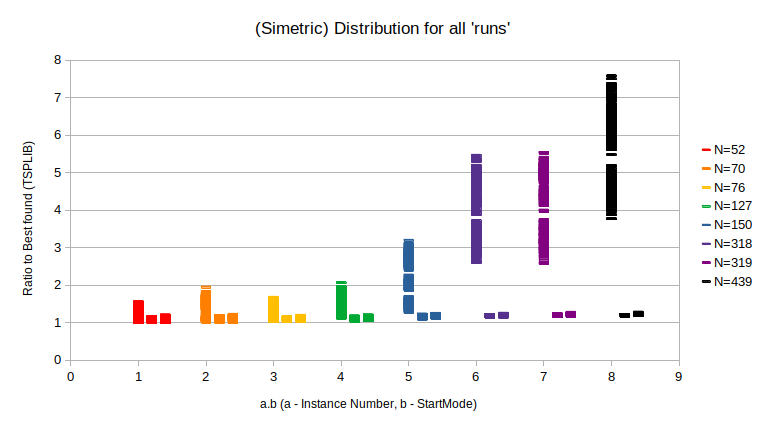
\includegraphics[scale=0.36]{simDistI}
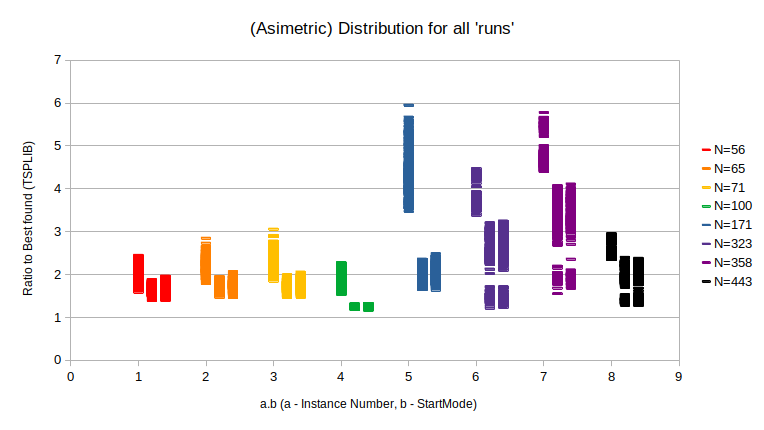
\includegraphics[scale=0.36]{asimDistI}

Z podanych wykresów można wyciągnąć dwa zasadnicze wnioski (które aplikują się zarówno do instancji symetrycznych, jak i asymetrycznych):
\begin{itemize}
	\item Jak widać, dla większych instancji algorytm startujący z rozwiązań losowych nie miał wystarczającej ilości czasu, aby dotrzeć do rozwiązań (w sensie wydajności) zbliżonych do pozostałych trybów startowania. Jednak dla instancji mniejszego rozmiaru, z samego tylko wykresu trudno byłoby powiedzieć, czy jego rozwiązania są rzeczywiście gorsze, chociaż  jasno widać, że mają one (o losowym starcie) znacznie większy rozrzut.
	\item Dla większych instancji, pomimo dużego rozrzutu danych, dla samych rozwiązań startujących z całkowicie losowej populacji można wyznaczyć dwie 'grupy', daltego też zaryzykujemy tu swierdzenie, że dla pozostałych trybów startu także to zachodzi (chociaż na razie tego nie widać)
\end{itemize}

\subsubsection{Rozrzut wyników dla poszczególnych instancji}
Pokażemy teraz dystrybucję wyniku względem liczby iteracji osobno dla każdej instancji. Jednak, nie zawrzemy tutaj wyników, które zostały otrzymane przez użycie całkowicie losowej populacji początkowej, ponieważ tak jak zauważyliśmy na poprzednich wykresach, odbiegają znacznie od pozostałych 2 trybów startujących.

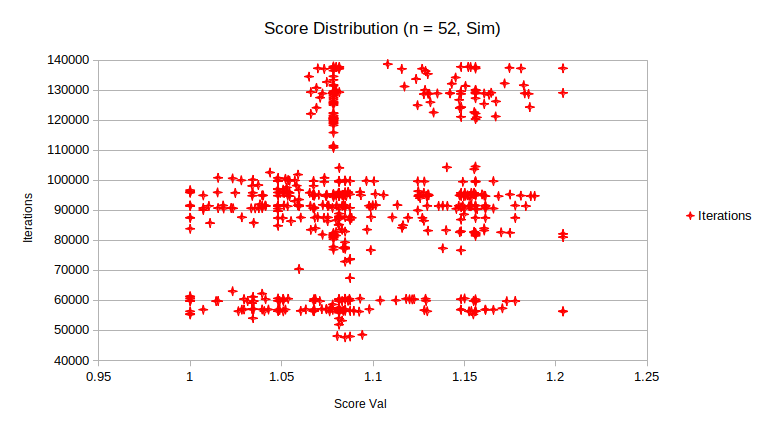
\includegraphics[scale=0.36]{simDist52}
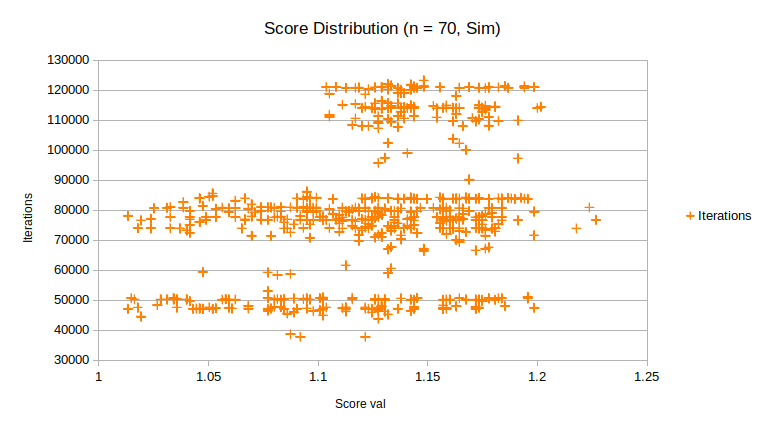
\includegraphics[scale=0.36]{simDist70}
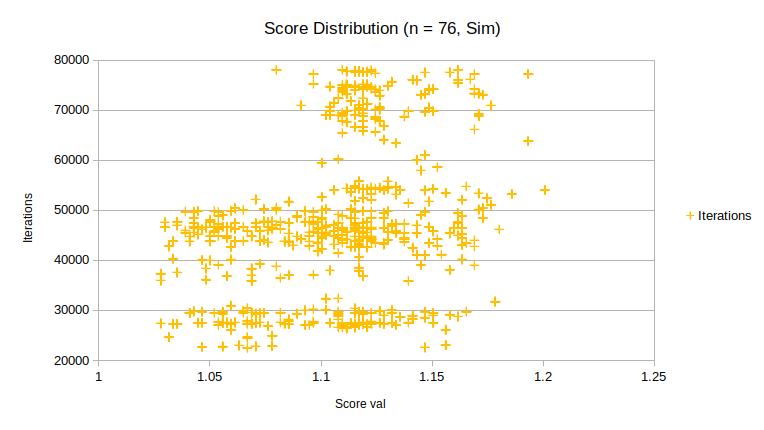
\includegraphics[scale=0.36]{simDist76}
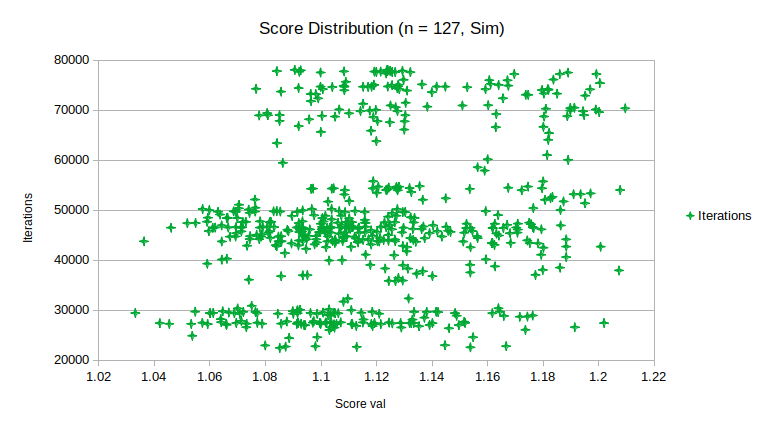
\includegraphics[scale=0.36]{simDist127}
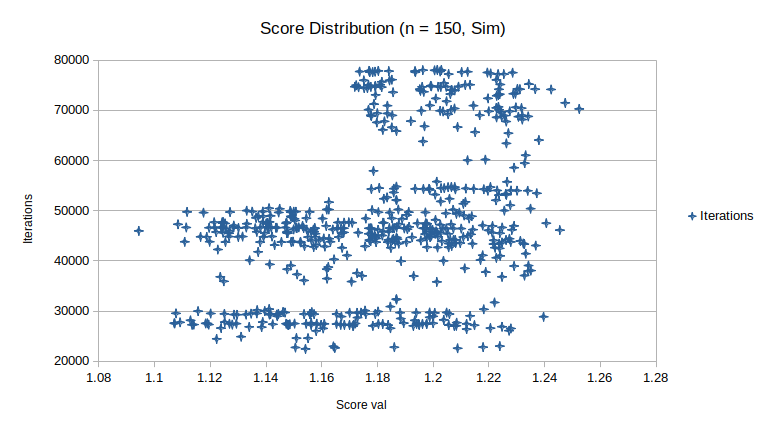
\includegraphics[scale=0.36]{simDist150}
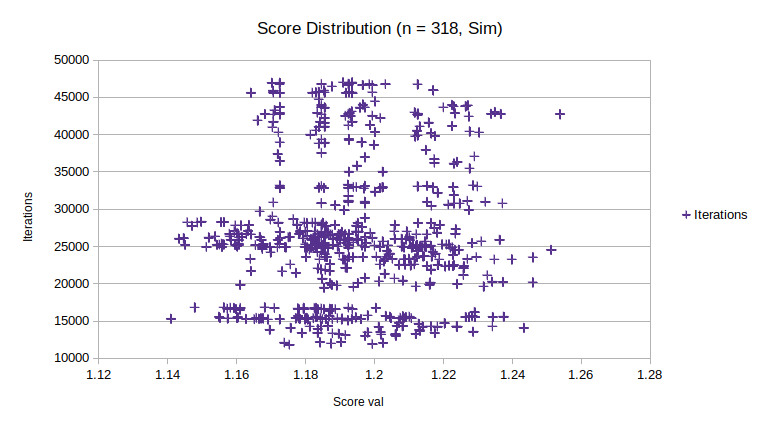
\includegraphics[scale=0.36]{simDist318}
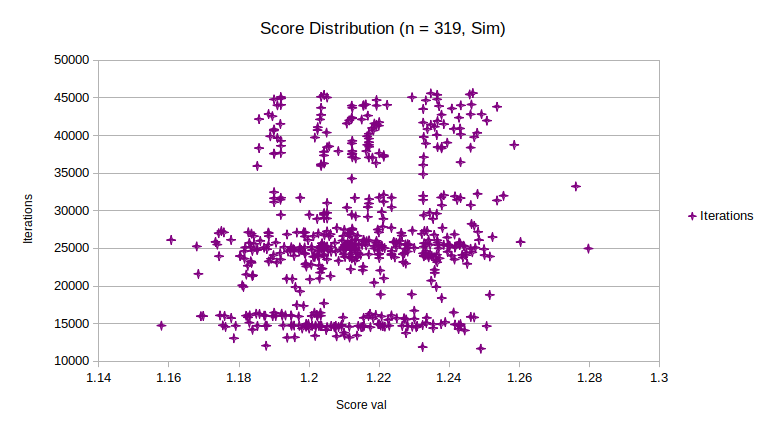
\includegraphics[scale=0.36]{simDist319}
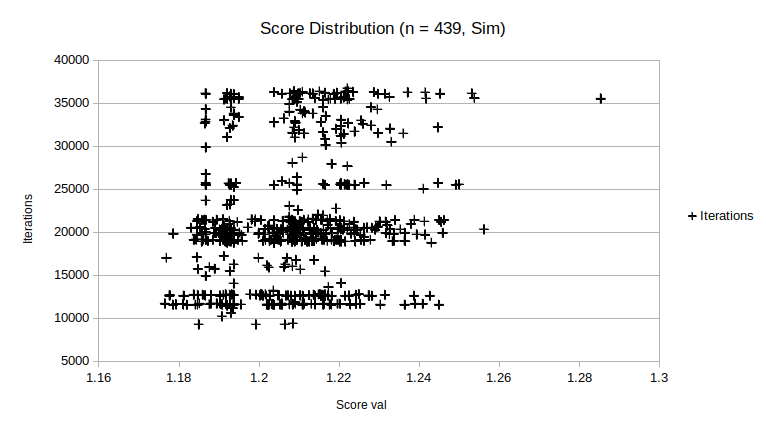
\includegraphics[scale=0.36]{simDist439}

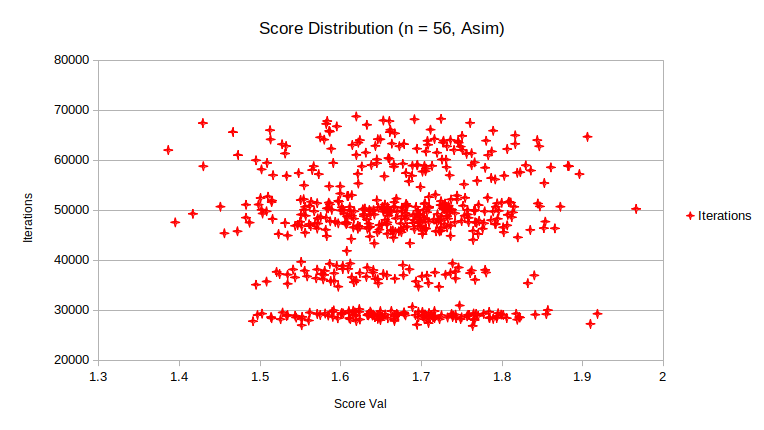
\includegraphics[scale=0.36]{asimDist56}
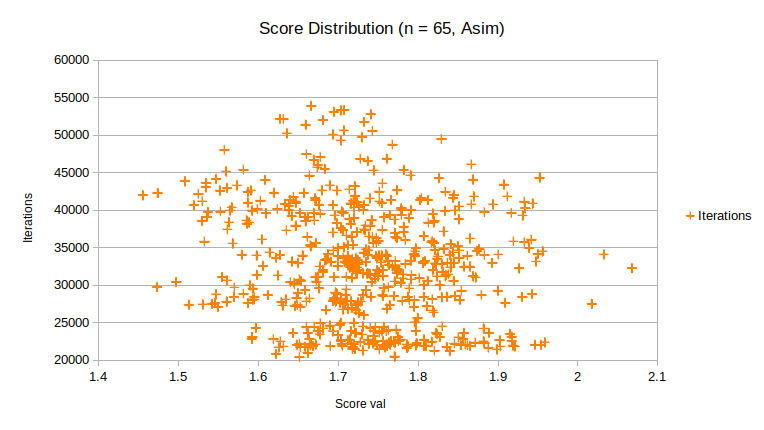
\includegraphics[scale=0.36]{asimDist65}
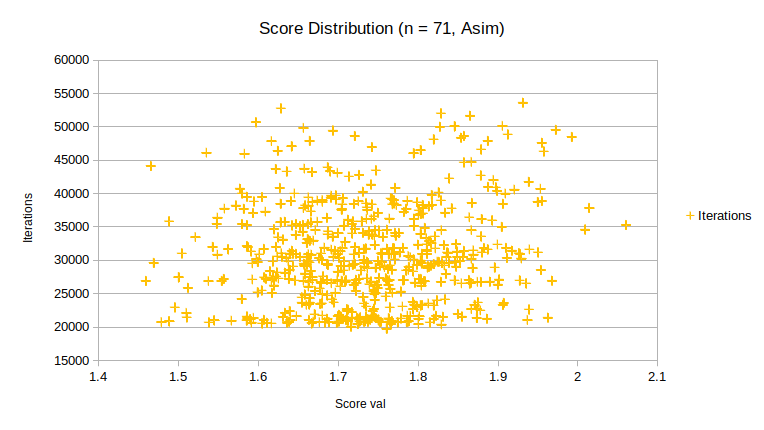
\includegraphics[scale=0.36]{asimDist71}
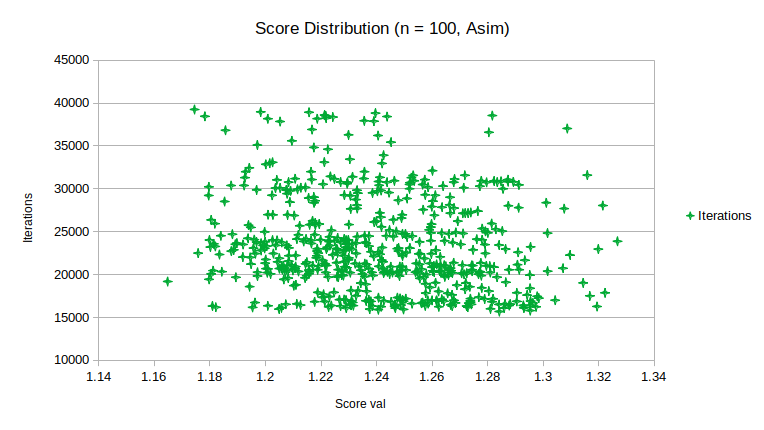
\includegraphics[scale=0.36]{asimDist100}
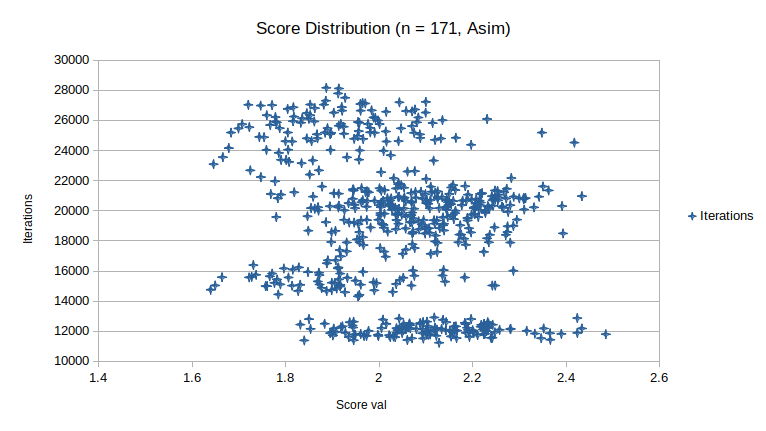
\includegraphics[scale=0.36]{asimDist171}
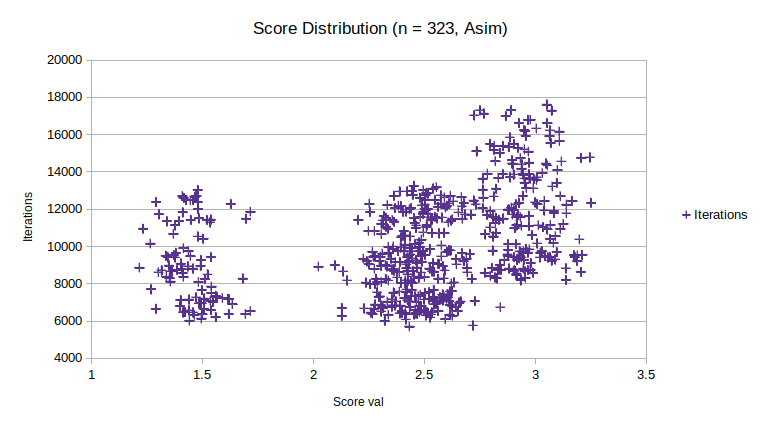
\includegraphics[scale=0.36]{asimDist323}
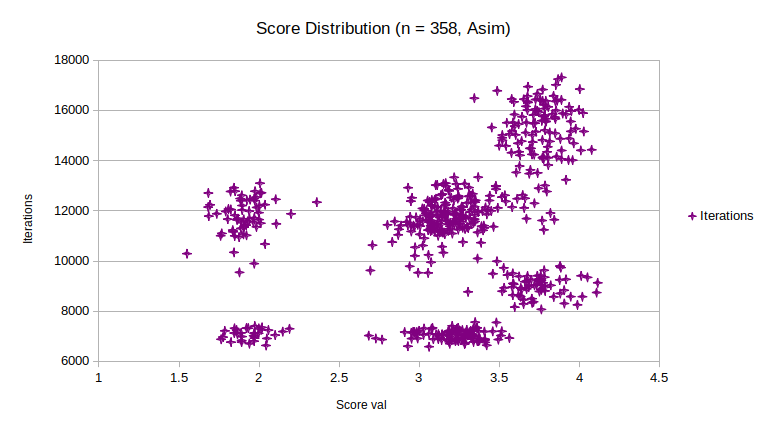
\includegraphics[scale=0.36]{asimDist358}
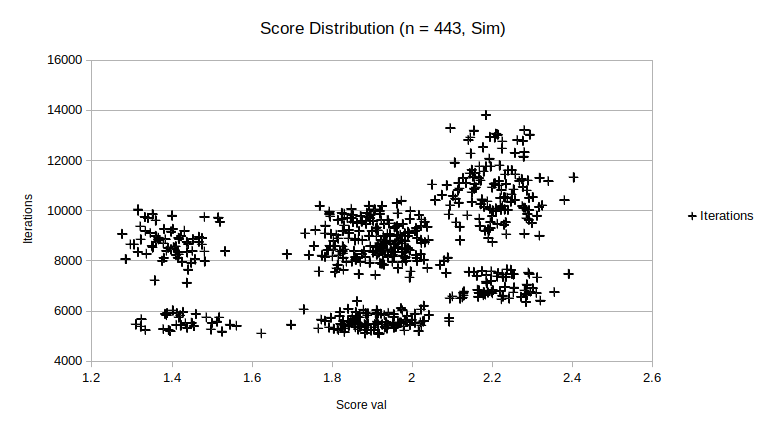
\includegraphics[scale=0.36]{asimDist443}

\newpage
Z tych wykresów wyciągnijmy jeszcze kilka wniosków:
\begin{itemize}
	\item Najbardziej rzuca się w oczyw dosyć wyraźna 'klasteryzacja' rozwiązań ( najbardziej w przypadku większych instancji) - co idealnie pokazuje, że konkretne kombinacje trybów bardzo różnie ze sobą działają ( i można dzięki temu wyznaczyć prosperujące)
	\item Pomimo znacznej różnicy w liczbie wykonanych iteracji, nie ma bezpośredniego związku między wynikiem - ozncza to, że są tryby, które bardzo 'szybko' znajdują rozwiązanie 'dobre', pomimo tego, że wykonanie pojedynczego kroku trwa o wiele dłużej.
	\item W miarę zwiększania się problemu instancji widać coraz wyraźniejsze różnice między poszczególymi kombinacjami (nie są nazwane, ale bardziej chodzi tutaj o zaakcentowanie wystepowania zjawiska)
	\item Widać również różnice dla wariantu symetrycznego, oraz asymetrycznego - drugie są o wiele bardziej 'skondensowane' mi układają się bardziej 'pasmowo' - może to wynikać z natury problemu - albo dane ruchy są wymagające, albo nie (W przypadku symetrycznych różnice są bardziej - niespodziewane - symetryczne)
\end{itemize}

\subsubsection{Tryby pod względem jednostkowym}
Pokażemy teraz tabele podsumowującą wszystkie instancje symetryczne, oraz asymetryczne, w której to zawrzemy informacje o minimum i średniej rozwiązań w rozbiciu o każdy tryb (to znaczy, że będziemy patrzeć na całą naszą przestrzeń rozwiązań, a następnie będziemy ją dzielić na rozwiązania względem danego trybu, zatem najpierw (w pierwszych 3 wierszach) podzielimy całość na 3 metody startowe, następnie całość podzielimy na 2 metody selekcji, itd.), z czego wyciągniemy informacje, jakie wartośći danych trybów są ogółem najlepsze gdy się nie bierze pod uwagę kombinacji innych.

\begin{table}[h!]
	\centering
	\begin{tabular}{c|c||c|c||c|c}
Tabela 1. \\
Tryb & Wartość trybu & Min (Sym) & Avg (Sym)  & Min (Asym) & Avg (Asym)\\
\hline
StartMode & 0 & 1 & 2.751 & 1.533 & 2.988\\
 & 1 & 1 & 1.144 & 1.175 & 1.981\\
 & 2 & 1 & 1.165 & 1.164 & 2.008\\
\hline
SelectionMode & 0 & 1 & 1.682 & 1.174 & 2.321\\
 & 1 & 1 & 1.691 & 1.164 & 2.331\\
\hline
MutMode & 0 & 1.020 & 1.562 & 1.164 & 2.275\\
 & 1 & 1 & 1.736 & 1.179 & 2.338\\
 & 2 & 1.067 & 1.851 & 1.174 & 2.336\\
 & 3 & 1 & 1.597 & 1.175 & 2.330\\
\hline
crossMode & 0 & 1.065 & 1.819 & 1.174 & 2.419\\
 & 1 & 1 & 1.616 & 1.180 & 2.277\\
 & 2 & 1 & 1.625 & 1.164 & 2.281\\
\hline
crossType & 0 & 1 & 1.697 & 1.178 & 2.326\\
 & 1 & 1 & 1.671 & 1.164 & 2.324\\
 & 2 & 1 & 1.692 & 1.174 & 2.328\\
	\end{tabular}
\end{table}

Z obu powyższych tabel możemy wyciągnąć następujące wnioski:
\begin{itemize}
	\item Możemy zaobserwować, że zaskakująco wiele kombinacji (ponieważ każdy tryb jednostkowo wchodzi w kilkadziesiąt innych) znalazło chociaż raz rozwiązanie optymalne! Jednak jak się przyjrzymy wcześniejszym wykresom, to zauważymy, że taka sytuacja wydarzyła się jedynie dla najmniejszej z rozpatrywanych instancji.
	\item Dalej widać, że pod względem średniej globalnej, dane tryby z osobna nie różnią się znacznie od siebie, dlatego też o wiele więcej informacji będziemy w stanie wyciągnąć z dalszej analizy.
\end{itemize}

\subsubsection{10 najlepszych kombinacji}
Teraz spójrzmy jeszcze na ranking 10 najlepszych zestawów parametrów zebranych ze wszystkich instancji.\\
Ranking stworzony został w następujący sposób:
\begin{itemize}
	\item W obrębie każdej instancji:
	\begin{itemize}
		\item Najpierw policzyliśmy minimum oraz średnią z 4 wywołań każdej kombinacji
		\item Później zsumowaliśmy ze sobą obie otrzymane wartości
		\item Następnie posortowaliśmy kombinacje rosnąco względem otrzymanej sumy
		\item Teraz przyporządkowaliśmy miejsca do otrzymanego porządku (przy dublowaniu któregoś z miejsc omijaliśmy kolejne: 32, 32, 34)	
	\end{itemize}
	\item W obrębie typu instancji (symetryczne / asymetryczne),  a później globalnie (wszystkie 16 razem)
	\begin{itemize}
		\item Zsumowaliśmy zajęte miejsca dla każdej kombinacji
		\item posortowaliśmy rosnąco otrzymując ostateczny 'ranking' dla wszystkich kombinacji w obrębie danego typu.	
	\end{itemize}
\end{itemize}

Oto 'główki' dla otrzymanych wyników (Ostatecznie wybraliśmy pierwszy rekord z każdej):
\begin{table}[h!]
	\centering
	\begin{tabular}{c||c|c|c|c|c||c|c}
Tabela 2.\\
Sym.\\
Id & StartMode & SelectionMode & MutMode & CrossMode & CrossType & Sum & Avg \\
\hline
107 & 1 & 0 & 3 & 2 & 2 & 98 & 12.25 \\
102 & 1 & 0 & 3 & 1 & 0 & 124 & 15.5 \\
106 & 1 & 0 & 3 & 2 & 1 & 127 & 15.875 \\
103 & 1 & 0 & 3 & 1 & 1 & 141 & 17.625 \\
142 & 1 & 1 & 3 & 2 & 1 & 161 & 20.125 \\
139 & 1 & 1 & 3 & 1 & 1 & 163 & 20.375 \\
140 & 1 & 1 & 3 & 1 & 2 & 188 & 23.5 \\
143 & 1 & 1 & 3 & 2 & 2 & 197 & 24.625 \\
138 & 1 & 1 & 3 & 1 & 0 & 202 & 25.25 \\
104 & 1 & 0 & 3 & 1 & 2 & 206 & 25.75 \\
	\end{tabular}
\end{table}

\begin{table}[h!]
	\centering
	\begin{tabular}{c||c|c|c|c|c||c|c}
Tabela 3.\\
Asym.\\
Id & StartMode & SelectionMode & MutMode & CrossMode & CrossType & Sum & Avg \\
\hline
77 & 1 & 0 & 0 & 1 & 2 & 193 & 24.125 \\
75 & 1 & 0 & 0 & 1 & 0 & 225 & 28.125 \\
149 & 2 & 0 & 0 & 1 & 2 & 227 & 28.375 \\
76 & 1 & 0 & 0 & 1 & 1 & 250 & 31.25 \\
115 & 1 & 1 & 0 & 2 & 1 & 267 & 33.375 \\
114 & 1 & 1 & 0 & 2 & 0 & 270 & 33.75 \\
112 & 1 & 1 & 0 & 1 & 1 & 274 & 34.25 \\
185 & 2 & 1 & 0 & 1 & 2 & 276 & 34.5 \\
80 & 1 & 0 & 0 & 2 & 2 & 278 & 34.75 \\
113 & 1 & 1 & 0 & 1 & 2 & 289 & 36.125 \\
	\end{tabular}
\end{table}

\begin{table}[h!]
	\centering
	\begin{tabular}{c||c|c|c|c|c||c|c}
Tabela 4.\\
Wspólne\\
Id & StartMode & SelectionMode & MutMode & CrossMode & CrossType & Sum & Avg \\
\hline
76 & 1 & 0 & 0 & 1 & 1 & 461 & 28.8125 \\
75 & 1 & 0 & 0 & 1 & 0 & 471 & 29.4375 \\
77 & 1 & 0 & 0 & 1 & 2 & 494 & 30.875 \\
115 & 1 & 1 & 0 & 2 & 1 & 494 & 30.875 \\
113 & 1 & 1 & 0 & 1 & 2 & 522 & 32.625 \\
112 & 1 & 1 & 0 & 1 & 1 & 536 & 33.5 \\
114 & 1 & 1 & 0 & 2 & 0 & 546 & 34.125 \\
103 & 1 & 0 & 3 & 1 & 1 & 579 & 36.1875 \\
116 & 1 & 1 & 0 & 2 & 2 & 590 & 36.875 \\
111 & 1 & 1 & 0 & 1 & 0 & 596 & 37.25 \\
	\end{tabular}
\end{table}

Na koniec jeszce taka uwaga: zaniechaliśmy zamieszczanie testów statystycznych, ponieważ każdy z badanych trybów był jednoznacznie 'dobry', albo bez znaczenia (jak na przykład StartMode = 1). Na koniec dodamy jeszcze tabelkę z pierwszymi 50 wynikami naszego rankingu, aby to podkreślić.

\newpage
\subsection{Poszukiwanie II - hiperparametry}
Po wyznaczeniu rokujących zestawów trybów, przeszliśmy do wyznaczenia jak najlepszych hiperparametrów. W tym celu wyznaczyliśmy 1 zestaw dla wariantu symetrycznego (Spec), 1 dla asymetrycznego (Spec), oraz 1 wspólny (Gen).\\
Poprzez metodę losowego próbkowania dla każdego hiperparametru (losowy z zakresu podanego zaraz), wykonaliśmy 100 kombinacji, gdzie każdą testowaliśmy 4 razy.\\
Badane instancje:
\begin{itemize}
	\item st70.tsp - sym.
	\item pr439.tsp - sym.
	\item ftv70.atsp - asym.
	\item rbg443.atsp - asym.
\end{itemize}
Badany zakres hiperparametrów:
\begin{itemize}
	\item populationSize : $[10 ; 100]$
	\item mutationThreshold : $[0.0 ; 1.0]$
	\item mutationIntensification : $[1 ; 20]$
	\item crossSize : $[2 ; 20]$
	\item crossCount : $[10 ; 200]$
\end{itemize}
Z przeprowadzonych eksperymentów otrzymaliśmy następujące wyniki:

\subsubsection{Rozrzut wyników dla poszczególnych instancji}
Na samym początku zaprezentujemy na wykresach, jak wygląda rozkład otrzymanych wyników dla każdej z badanych instancji.

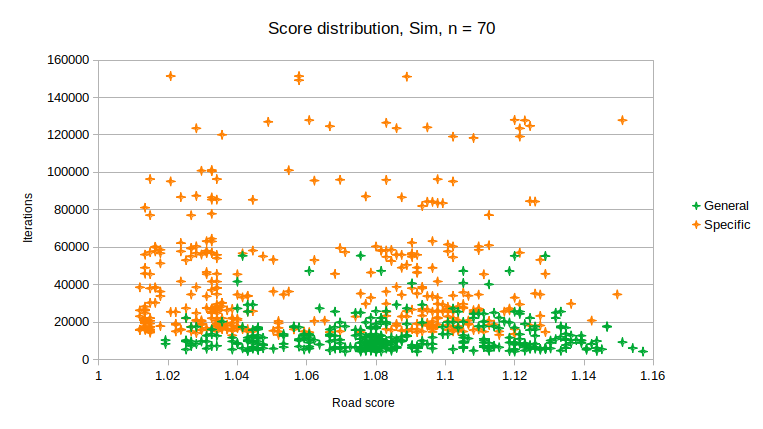
\includegraphics[scale=0.36]{parDistSim70}
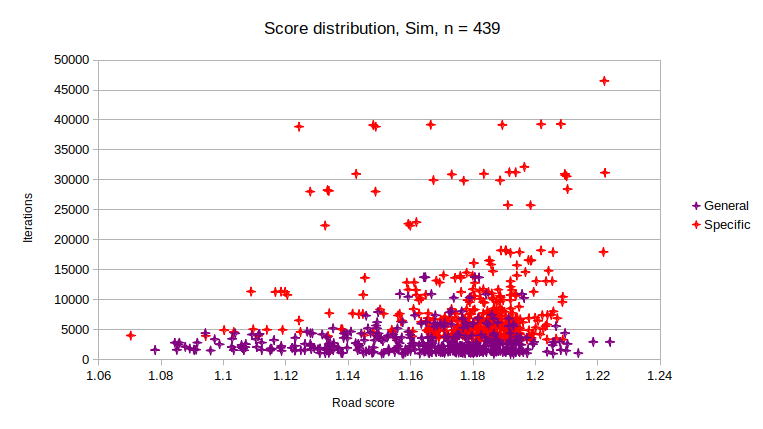
\includegraphics[scale=0.36]{parDistSim439}
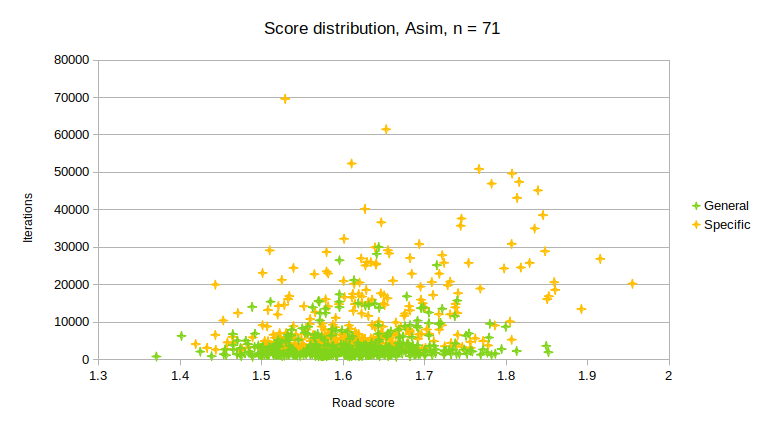
\includegraphics[scale=0.36]{parDistAsim71}
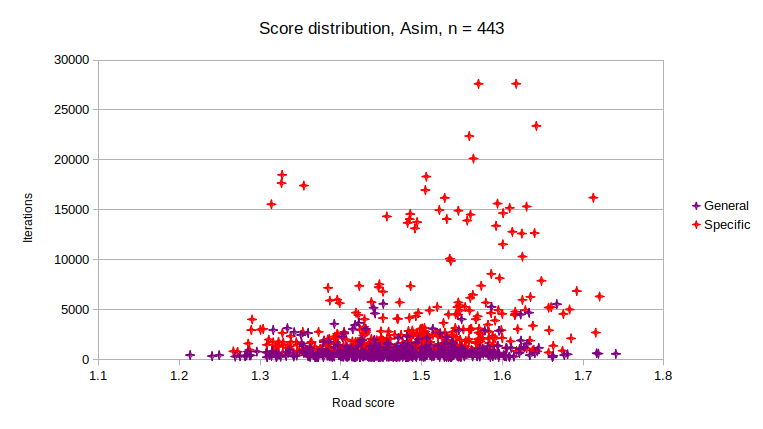
\includegraphics[scale=0.36]{parDistAsim443}

\newpage
Z powyższych wykresów spróbujmy teraz wyciągnąć kilka wniosków:
\begin{itemize}
	\item Jak widać dla wariantu symetrycznego, dla rozmiaru wielkości 70 o wiele lepiej zadziałał zestaw trybów deykowany do tych instancji, jednakże dla rozmiaru 439, o wiele lepiej zachował się zestaw ogólny. Przez sformułowanie 'lepiej' rozumiemy tutaj wartości częściej osiągane bliższej wartości rozwiązania najlepszego.
	\item Dla wariantu symetrycznego widać również, że dla każdej instancji zestaw danych ogólny wykonywał mniej iteracji (koncentracja w 'dolnej' części wykresu). Może być to powodowane tym, że jest on uwarunkowany po części parametrem \textit{crossCount}, który to mówi o liczbie wykonywanych krzyżowań - widzimy tutaj zatem 'średnią' zależność tego parametru od wykonanej liczby iteracji.
	\item Ogólny wniosek mamy zatem taki (i powtórzymy go zapewne przy okazji dalszej analizy): dla naszej implementacji różne zestawy trybów będą się inaczej zachowywały dla każdej instancji, zatem najlepszą metodą byłby dobór wszystkich trybów i parametrów do każdej instancji z osobna.
	\item Dopowiedzmy jesze tylko, że dla wariantu asymetrycznego o dziwo oba warianty były dosyć zbalansowane pod względem wydajności, co zresztą widać na rozrzucie danych
\end{itemize}

\subsubsection{Wykresy wobec parametrów dla każdej instancji}
W tej części pokażemy wykresy w rozbiciu o każdy parametr z osobna (traktujemy teraz wszystkie 100 przeszukiwań jako 1 zbiór i dzielimy go względem danego parametru). Pominiemy jednak wykresy dla parametru crossCount, ponieważ dla zestawów specyficznych dla danego typu (a/symetryczne) nie bierze on udziału):

\subsubsection*{Symetryczne}
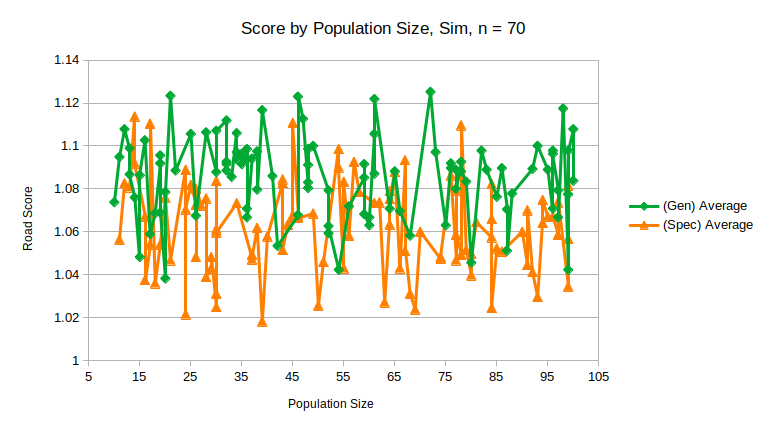
\includegraphics[scale=0.36]{pSSim70}
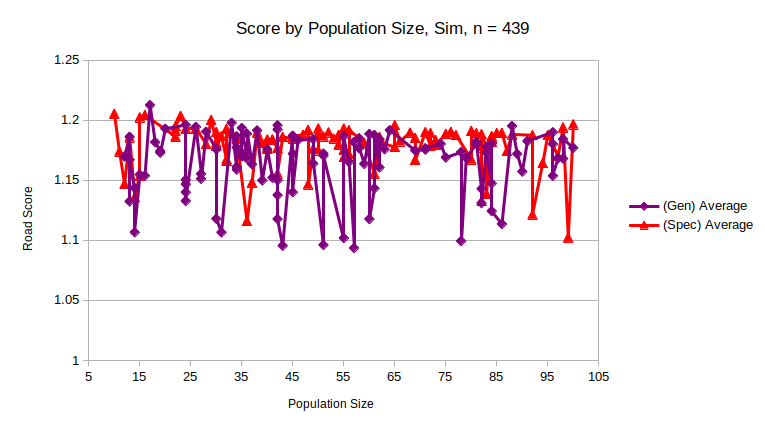
\includegraphics[scale=0.36]{pSSim439}
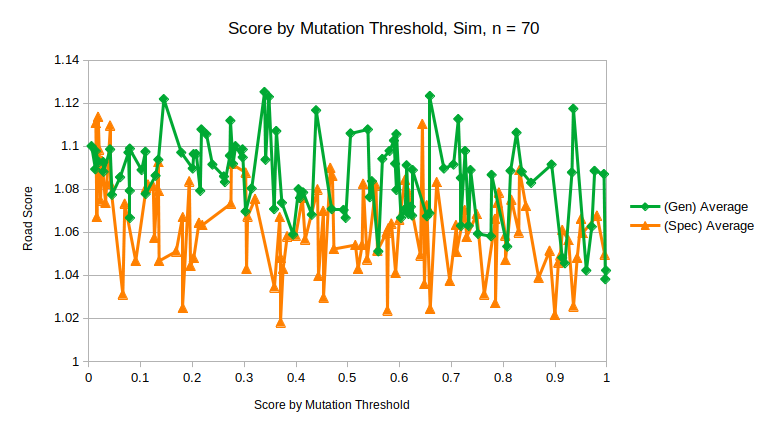
\includegraphics[scale=0.36]{mTSim70}
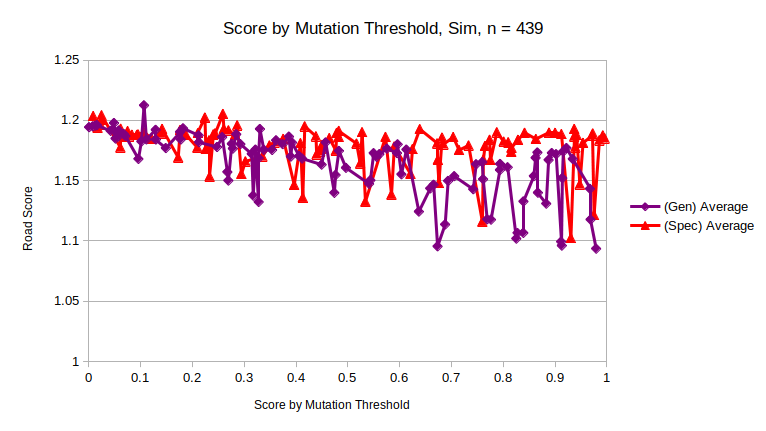
\includegraphics[scale=0.36]{mTSim439}
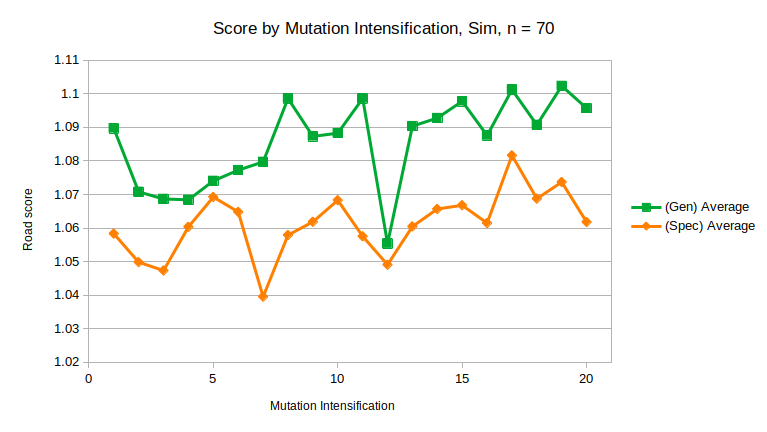
\includegraphics[scale=0.36]{mISim70}
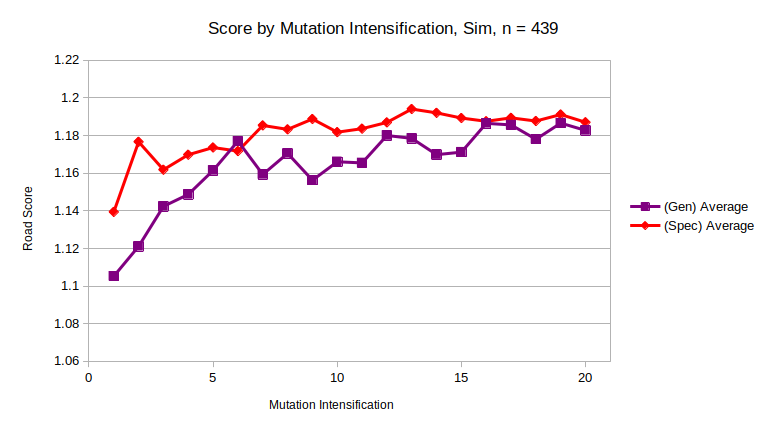
\includegraphics[scale=0.36]{mISim439}
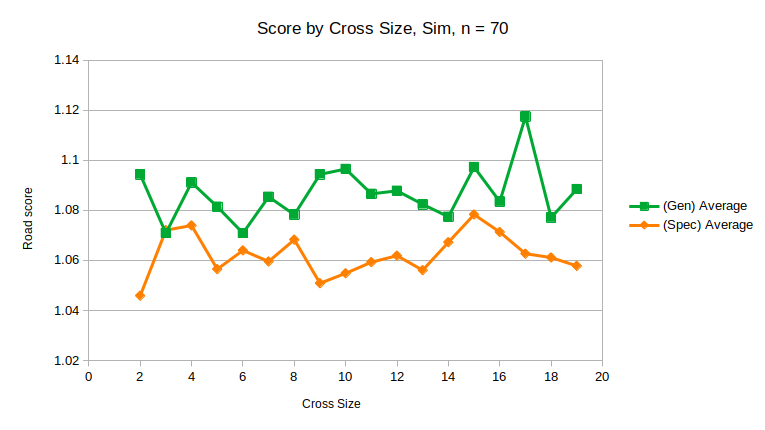
\includegraphics[scale=0.36]{cSSim70}
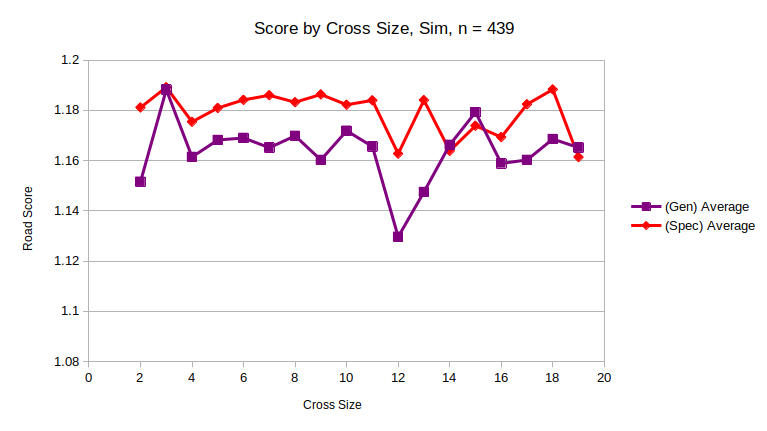
\includegraphics[scale=0.36]{cSSim439}

\subsubsection*{Asymetryczne}
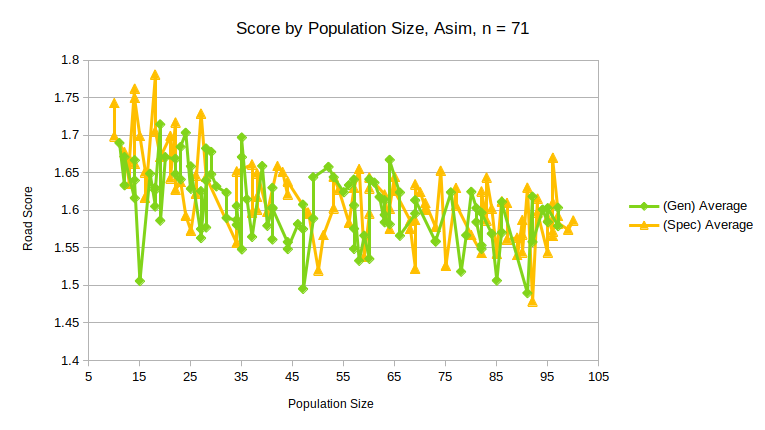
\includegraphics[scale=0.36]{pSAsim71}
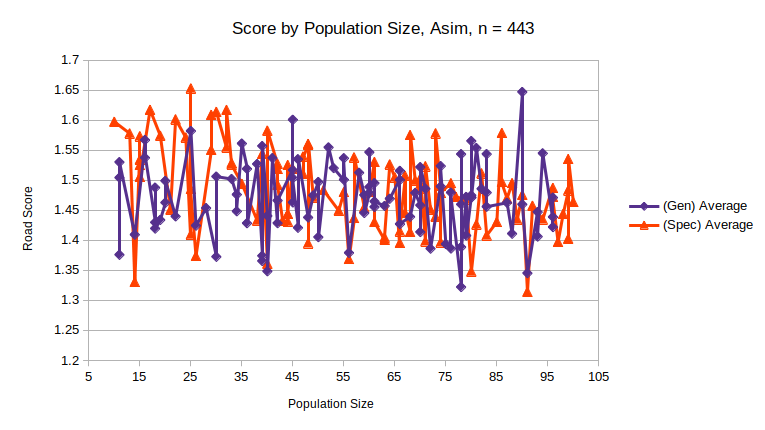
\includegraphics[scale=0.36]{pSAsim443}
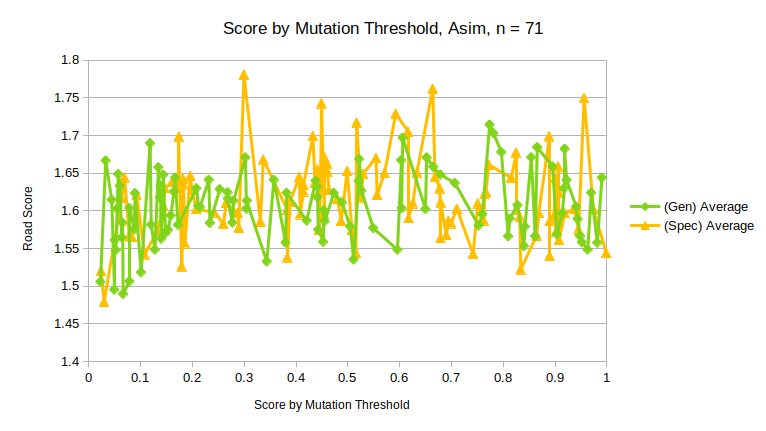
\includegraphics[scale=0.36]{mTAsim71}
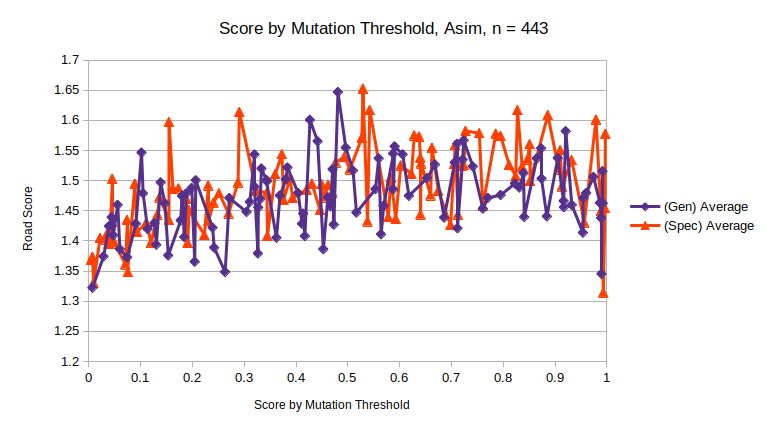
\includegraphics[scale=0.36]{mTAsim443}
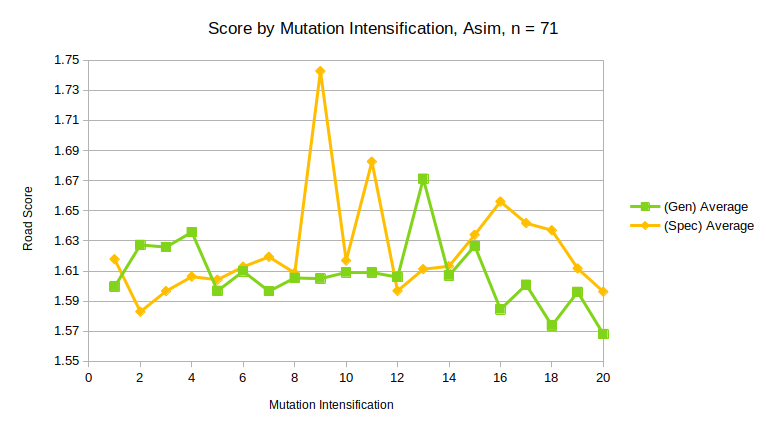
\includegraphics[scale=0.36]{mIAsim71}
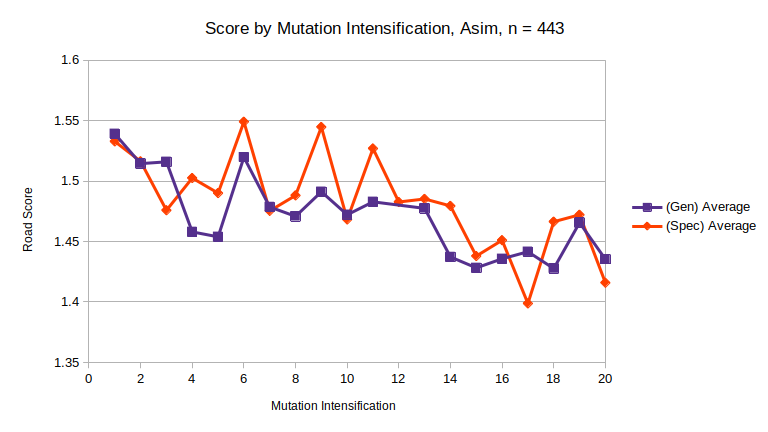
\includegraphics[scale=0.36]{mIAsim443}
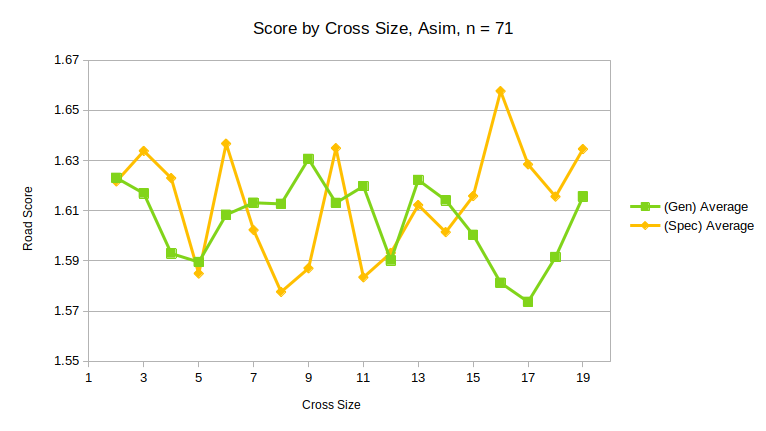
\includegraphics[scale=0.36]{cSAsim71}
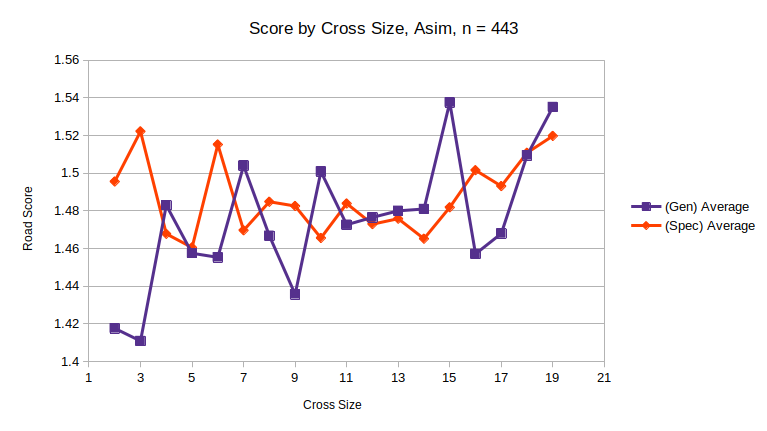
\includegraphics[scale=0.36]{cSAsim443}

Z powyższych wykresów spróbujmy wyciągnąć kilka wniosków:
\begin{itemize}
	\item Powtórzmy tutaj na początek wniosek z poprzedniej części, a konkretnie, że mimo wszystko zestawy trybów znacznie różnią się od siebie wydajnością (i wpływem na ogólny wynik hiperparametrów) w zależności od wybranej instancji.
	\item Wydawać by się mogło, że najmniejszy wpływ na wyniki ma wielkość populacji początkowej (na wszystkich wykresach wyniki są dosyć 'zbalansowane' niezależnie od tej wartości)
	\item Dla instancji mniejszego rozmiaru widzimy ogólnie mniejszą zależność od hiperparametrów, chociaż dla obu wariantów możemy zauważyć, że optimum dla intensyfikacji jest w okolicach \textit{magicznej 7}, natomiast dla crossSize w okolicach 9.
	\item Dla instanji większego rozmiaru możemy zauważyć, że zwiększanie prawdopodobieństwa mutacji znacznie poprawia jakość rozwiązania, jednakże zwiększanie intensyfikacji ją pogarsza. Można zatem powiedzieć, że najlepiej jest 'często mutować, ale delikatnie'. Natomiast wielkość parametru crossSize wacha się w okolicy 12.
\end{itemize}

\subsubsection{5 najlepszych}
Teraz spójrzmy na ranking 5 najlepszych zestawów parametrów dla każdej z badanych instancji:

\begin{table}[h!]
	\centering
	\begin{tabular}{c||c|c|c|c||c|c|c|c}
Tabela 5.\\
Symetryczne & \multicolumn{4}{c}{n = 70} &\multicolumn{4}{c}{n = 439}\\
Miejsce & popSize & mutThresh & mutInt & crosSize & popSize & mutThresh & mutInt & crosSize \\
\hline
1 & 39 & 0.370261 & 13 & 19 & 51 & 0.912935 & 1 & 11 \\
2 & 69 & 0.576427 & 12 & 7 & 57 & 0.979261 & 2 & 2 \\
3 & 84 & 0.658883 & 19 & 8 & 43 & 0.673103 & 1 & 12 \\
4 & 24 & 0.899584 & 12 & 13 & 78 & 0.911664 & 1 & 12 \\
5 & 50 & 0.935501 & 7 & 5 & 55 & 0.825131 & 1 & 14 \\

	\end{tabular}
\end{table}

\begin{table}[h!]
	\centering
	\begin{tabular}{c||c|c|c|c||c|c|c|c}
Tabela 6.\\
Asymetryczne & \multicolumn{4}{c}{n = 71} &\multicolumn{4}{c}{n = 443}\\
Miejsce & popSize & mutThresh & mutInt & crosSize & popSize & mutThresh & mutInt & crosSize \\
\hline
1 & 91 & 0.0661295 & 18 & 17 & 91 & 0.993212 & 19 & 12 \\
2 & 15 & 0.0222585 & 14 & 4 & 78 & 0.00685312 & 17 & 3 \\
3 & 92 & 0.0293365 & 20 & 8 & 91 & 0.989566 & 16 & 5 \\
4 & 47 & 0.0490319 & 10 & 17 & 80 & 0.0753719 & 10 & 4 \\
5 & 59 & 0.383063 & 5 & 7 & 93 & 0.1842 & 10 & 3 \\

	\end{tabular}
\end{table}

I wyciągnijmy z nich parę wniosków:
\begin{itemize}
	\item Jak widzimy, dane otrzymane w tabeli nawet pokrywają się po części z tym, co zaobserwowaliśmy na wykresach, a konkretnie, a zwłasza to widać dla instancji 'dużych' i parametów związanych z mutacją (często, acz lekko).
	\item Dla instancji 'mniejszych' (przypomnijmy że zauważyliśmy na wykresach, że wyniki wydają się bardziej zbalansowane) dane w tabeli bardziej się różnią od siebie (większy rozrzut pomimo wzięcia tylko pierwszej 5), i powiedzmy, że ranking wydaje się nieco bardziej 'losowy' - ale dalej nam determiniuje 'zwycięzcę'
\end{itemize}

\subsubsection{Ostatecznie wybrane najlepsze}
Tak jak wcześniej powiedzieliśmy, nie można jednoznacznie wyznaczyć najlepszyych hiperparametrów dla całej metody, jednakże możemy wyznaczyć najlepszy zestaw danych dla poszczególnych instancji. Dlatego tak właśnie teraz postąpimy, i w dalszych eksperymentach będziemy używać następujących zestawów:

\begin{table}[h!]
	\centering
	\begin{tabular}{c||c|c|c|c|c||c|c|c|c}
Tabela 7. & \multicolumn{5}{c}{Tryby} &\multicolumn{4}{c}{Hiperparametry}\\
Instancja & Start & Sel. & Mut. & CrossM & CrossT & popSize & mutThresh & mutInt & crosSize \\
\hline
Sym70 & 1 & 0 & 3 & 2 & 2 & 39 & 0.370 & 13 & 19\\
Sym439 & 1 & 0 & 0 & 1 & 1 & 51 & 0.913 & 1 & 11\\
Asym71 & 1 & 0 & 0 & 1 & 2 & 91 & 0.067 & 18 & 17\\
Asym443 & 1 & 0 & 0 & 1 & 2 & 91 & 0.993 & 19 & 12\\

	\end{tabular}
\end{table}

\subsection{Badanie wpływu zastosowania 'lokalnej poprawy'}
Przy zastosowaniu wyników z 2 poprzednich eksperymentów postanowiliśmy zbadać wpływ działania mechanizmu 'lokalnej poprawy' na wyniki.\\\\
Badaliśmy te same 4 instancje, co w przypadku poszukiwania hiperparametrów, dlatego że jak się nam udało ustalić, najlepiej jest dobierać je do każdej instancji z osobna.\\\\
\textit{Lokalna poprawa} - z pewnym prawdopodobieństwem (określanym parametrem \textit{enhanceChance}) po skończonej mutacji (czyli po szystkich iteracjach) na osobniku wykonujemy algorytm lokalnej poprawy, czyli iteracyjnie przechodzimy przez piątki kolejnych miast i tak modyfikujemy trasę, aby w każdej z tych iteracji przejście było minimalne - zatem najpierw 'poprawiamy' miasta 1-5, potem 2-6 itd. Takich możliwych przejść jest 6 (ponieważ zaczynamy zawsze z 1 i kończymy na 5), zatem jest to w miarę szybkie (dzieje się w czasie liniowym względem liczby miast) i nie powinno znacząco wpływać na liczbę wykonywanych iteracji.\\\\
W testach wykonaliśmy 10 powtórzeń dla każdej wartości parametru z zakresu $[0.05 ; 1.0]$ ze skokiem o $0.05$. Wyniki przedstawmy na wykresach (będziemy pokazywali średnią, oraz najlepszy usyzkany wynik):

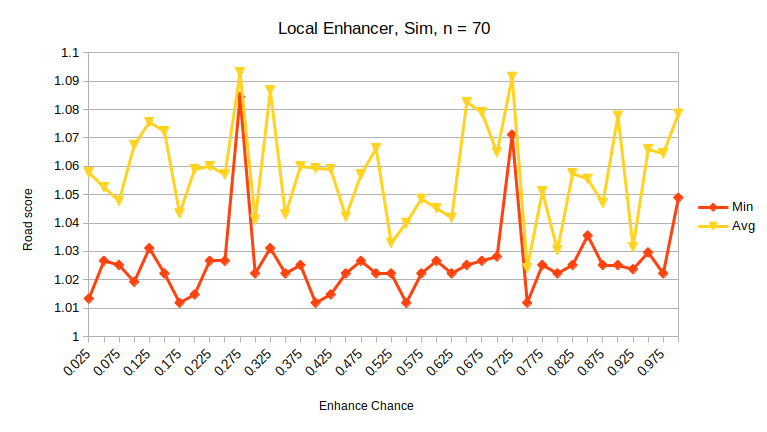
\includegraphics[scale=0.36]{locEnhSim70}
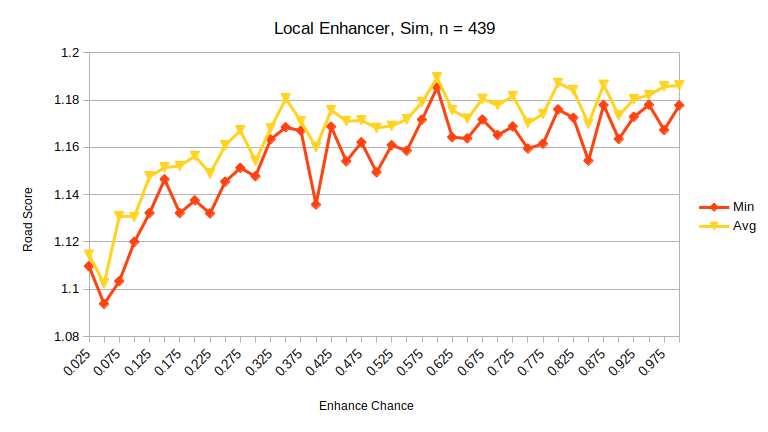
\includegraphics[scale=0.36]{locEnhSim439}
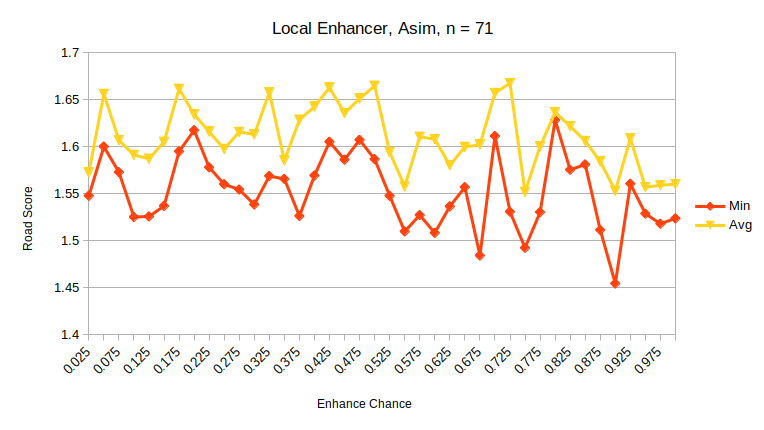
\includegraphics[scale=0.36]{locEnhAsim71}
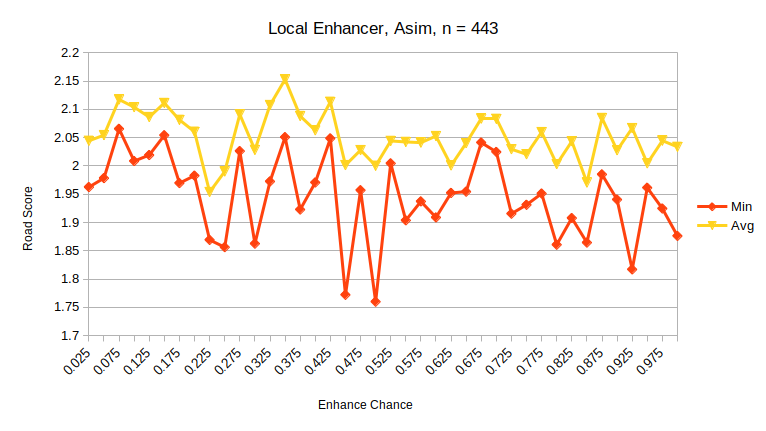
\includegraphics[scale=0.36]{locEnhAsim443}

Zamieśćmy jeszcze, jak wygląda wykres średniej liczby wykonanych iteracji względem badanego parametru:

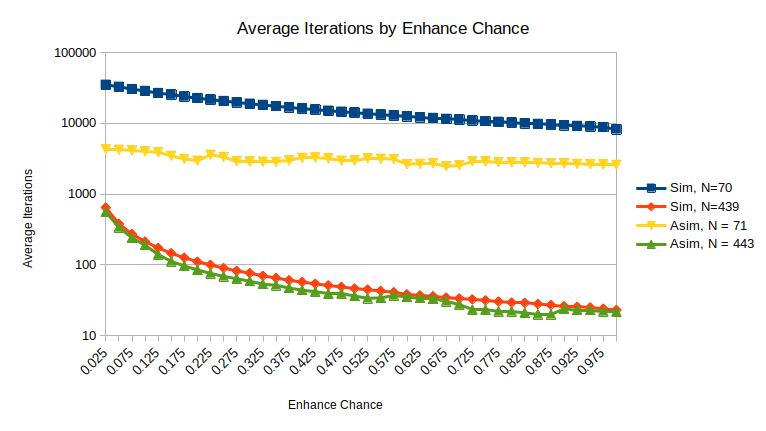
\includegraphics[scale=0.72]{locEnhIter}

Analiza tutaj jest dosyć prosta i oczywista: Parametr ten nie wpływa zbyt korzystnie na rozwiązanie, a czasem nawet czas poświęcony na jego wykonywanie sprawia, że wykonujemy znacznie mniej iteracji, przez co nie nadążamy z dotarciem do rozwiązań 'względnie dobrych'

\subsection{Badanie wpływu 'wieku' osobników}
Eksperyment analogiczny do poprzedniego (w sensie metodologii, wyboru instancji i parametrów), jednak tym razem badaliśmy wpływ zastosowania wieku na rozwiązanie. Oznaczyliśmy go jako \textit{AgeMax}, przy czym oznacza on, że osobnik będący w populacji dłużej niż \textit{AgeMax} w procesie selekcji jest 'usuwany' z populacji. Zastosowaliśmy tutaj jednak pewną formę elitaryzmu, ponieważ podczas każdej selekcji 'zerujemy' wiek najlepszego osobnika (Najlepszy ma prawo \textit{Picia ze źródła wiecznej młodości}), dzięki czemu go nie tracimy.\\
W testach wykonaliśmy 10 powtórzeń dla każdej wartości z zakresu $[1 ; 20]$, a wyniki przedstawiamy na wykresach:

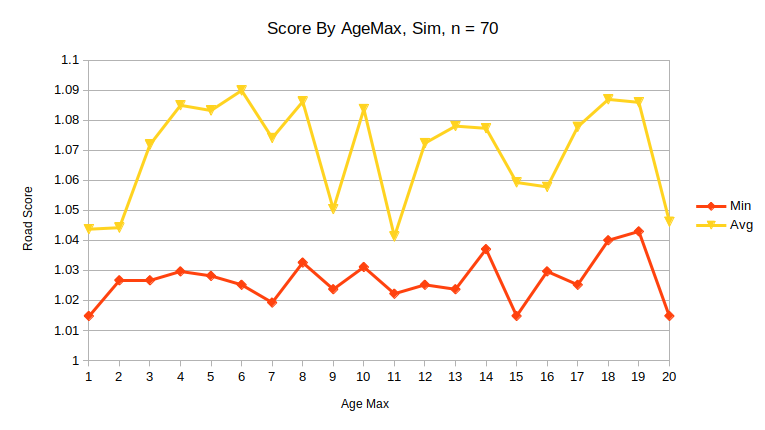
\includegraphics[scale=0.33]{ageSim70}
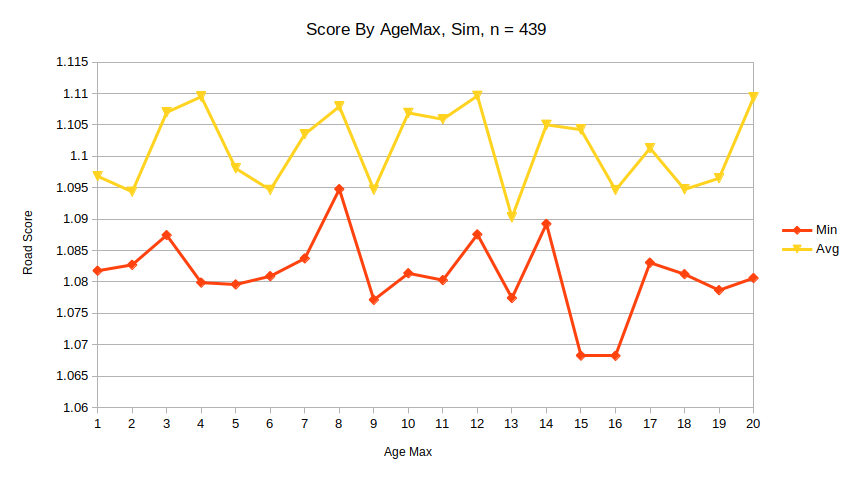
\includegraphics[scale=0.33]{ageSim439}
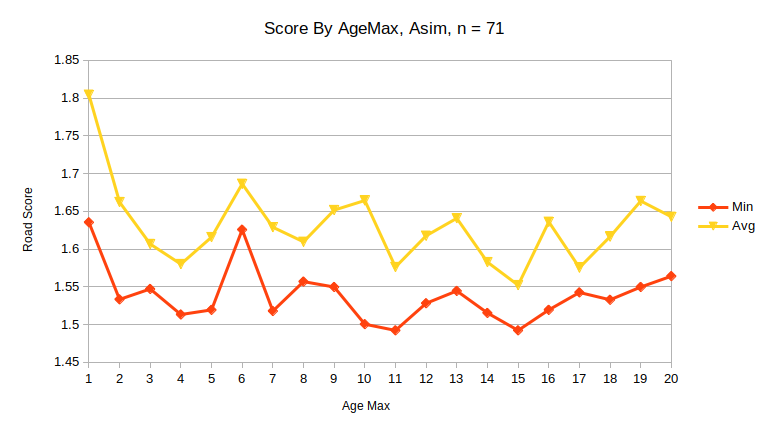
\includegraphics[scale=0.33]{ageAsim71}
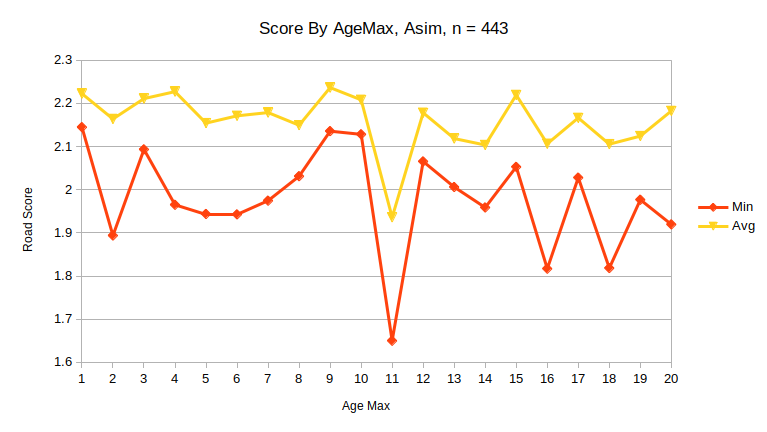
\includegraphics[scale=0.33]{ageAsim443}

Zamieśćmy jeszcze, jak wygląda wykres średniej liczby wykonanych iteracji względem badanego parametru:

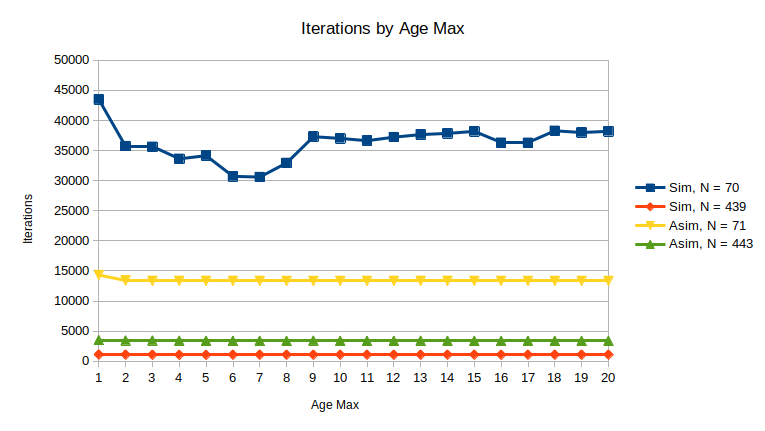
\includegraphics[scale=0.72]{ageIter}

\newpage
A teraz przeanalizujmy otrzymane wyniki:
\begin{itemize}
	\item Z liczby iteracji widać, że nie wpływa tutaj to znacząco na poziom zaawansowania populacji, zatem można stosować ten parametr 'wstępnie bezstratnie'
	\item Pomimo nieco losowego rozrzutu, to widzimy zadziwiającą zależność w obrębie jednego rodzaju (a/symetryczne), a konkretnie lokalne minima dla wartości odpowiednio 15 oraz 11
	\item Stwierdzamy zatem, że mimo wszystko ten parametr warto używać, i będziemy z niego korzystali.
\end{itemize}

\subsection{Porównanie najlepszych wyników z algorytmem TabuSearch}
Aby jakoś porównać działanie naszego algorytmu, zestawimy go tutaj z zaimplementoanym algorytmem \textit{TabuSearch}, gdzie Tabu będzie miało następujące parametry:
\begin{itemize}
	\item rozwiązanie startowe - najlepsze z losowych znalezionych w czasie 1 sekundy
	\item Wielkość listy Tabu - $\sqrt{n} + 2$
	\item Liczba iteracji bez poprawy: $\frac{(|LT| * 2 + 1) * 3}{2}$
	\item Otoczenie rotacyjne (Cykliczne zmiany między otoczeniami \textit{Invert}, \textit{Insert}, \textit{Swap})
	\item Kik rotacyjny (jak wyżej)
	\item Wielkość Kik'a = 7
	\item Korzystanie z mechanizmu Listy Długoterminowej
\end{itemize}
Natomiast \textit{Genetic} otrzymane z eksperymentów z poszukiwaniami. Jendakże, aby nie przeprowadzać pponownie poszukiwania najlepszych hiperparametrów dla każdej instancji, przyjęliśmy założenia, że wprowadzimy 1 'uśrednione' dla wszystkich (ale w dalszym ciąg rozróżniamy symetryczne i asymetryczne):
\begin{itemize}
	\item Symetryczne:
		\begin{itemize}
			\item startMode = 1
			\item selectionMode = 0
			\item mutMode = 3
			\item crossMode = 2
			\item crossType = 2
			\item populationSize = 45
			\item mutationThreshold = 0.64
			\item mutationIntensification = 13
			\item crossSize = 19
			\item crossCount = 177
    		\item enhanceChance = 0.01
    		\item ageMax = 15
		\end{itemize}
	\item Asymetryczne:
		\begin{itemize}
			\item startMode = 1
			\item selectionMode = 0
			\item mutMode = 0
			\item crossMode = 1
			\item crossType = 2
    		\item populationSize = 91
    		\item mutationThreshold = 0.99
			\item mutationIntensification = 18
			\item crossSize = 12
			\item crossCount = 176
    		\item enhanceChance = 0.01
    		\item ageMax = 11
		\end{itemize}
\end{itemize}
Testowaliśmy każdą z 16 badanych instancji, oraz każdemu z algorytmów daliśmy budżet czasu równy 90 sekund (Zatem Tabu działał przez 89). Aby jednak dać jakąś szansę (i odrobinę zredukować losowość) algorytmowi genetycznemu, wykonaliśmy dla niego 3 iteracje po 30 sekund, a następnie wybraliśmy najlepszy. W ten sposób jego wyniki mają szansę być nieco bardziej miarodajne. Wyniki przedstawmy w tabeli:

\begin{table}[h!]
	\centering
	\begin{tabular}{c||c|c|c}
Tabela 8.\\
Instancje & Wynik Tabu & Najlepszy Gen & Stosunek G:T\\
\hline
Sim, 52 & 7542 & 7772 & 1.03049588968443 \\
Sim, 70 & 676 & 696 & 1.02958579881657 \\
Sim, 76 & 550 & 564 & 1.02545454545455 \\
Sim, 127 & 118921 & 125369 & 1.05422086931661 \\
Sim, 150 & 26899 & 28935 & 1.07569054611696 \\
Sim, 318 & 172089 & 47532 & 0.276205916705891 \\
Sim, 318 & 202317 & 47565 & 0.235101350850398 \\
Sim, 439 & 1144057 & 124299 & 0.108647558644368 \\
Asim, 56 & 1660 & 2058 & 1.23975903614458 \\
Asim, 65 & 2032 & 2438 & 1.1998031496063 \\
Asim, 71 & 2162 & 2531 & 1.17067530064755 \\
Asim, 100 & 37931 & 42574 & 1.12240647491498 \\
Asim, 171 & 3617 & 5123 & 1.41636715510091 \\
Asim, 323 & 2243 & 2742 & 1.22246990637539 \\
Asim, 358 & 2823 & 3407 & 1.20687212185618 \\
Asim, 443 & 5461 & 5730 & 1.04925837758652 \\


	\end{tabular}
\end{table}

\begin{itemize}
	\item Jak widzimy, dla mniejszych instancji Tabu okazało się znacznie lepsze, co tłumaczymy tutaj po części ulosowieniem metody \textit{Genetic}
	\item Jednakże mamy 'anomalię' dla większych instancji symetrycznych, w postaci znacznie gorzszego wyniku dla Tabu. Tłumaczymy tutaj to jednak tym, że startowało ono z rozwiązań praktycznie losowych, oraz korzystało z listy długoterminowej, zatem zwyczajnie nie zdążyło dotrzeć do rozwiązań porównywalnych do \textit{Genetica}.
\end{itemize}

\subsection{Badania nad Modelem Wyspowym}
Model wyspowy zaimplementowano w następujący sposób:
\begin{itemize}
	\item Każda z wysp prowadzi własną instancję algorytmu genetyczne na pojedyńczym rdzeniu procesora, wyjściowa populacja losowa, parametry (wybrane najlepsze z uprzednich testów):
	\begin{itemize}
		\item populationSize = 50
		\item mutationIntensification = 13
		\item crossSize = 1
		\item crossCount = 177
		\item crossMode = 1
		\item mutMode = 0
		\item crossType = 1
		\item selectionMode = 0
    	\item mutationThreshold = 0.6
    	\item time = 30.0
	\end{itemize}
	\item po ustalonej liczbie iteracji, z każdej z wysp zabierano $k$ osobników, po czym z powstałej puli w losowy sposób wysyłano ich z powrotem na wyspy
\end{itemize}
Badania przeprowadzono na instancji st70.tsp, każda kombinacja parametrów została uruchomiona trzykrotnie, a wynik został uśredniony.
\subsubsection*{Wpływ długości interwału pomiędzy mieszaniem}
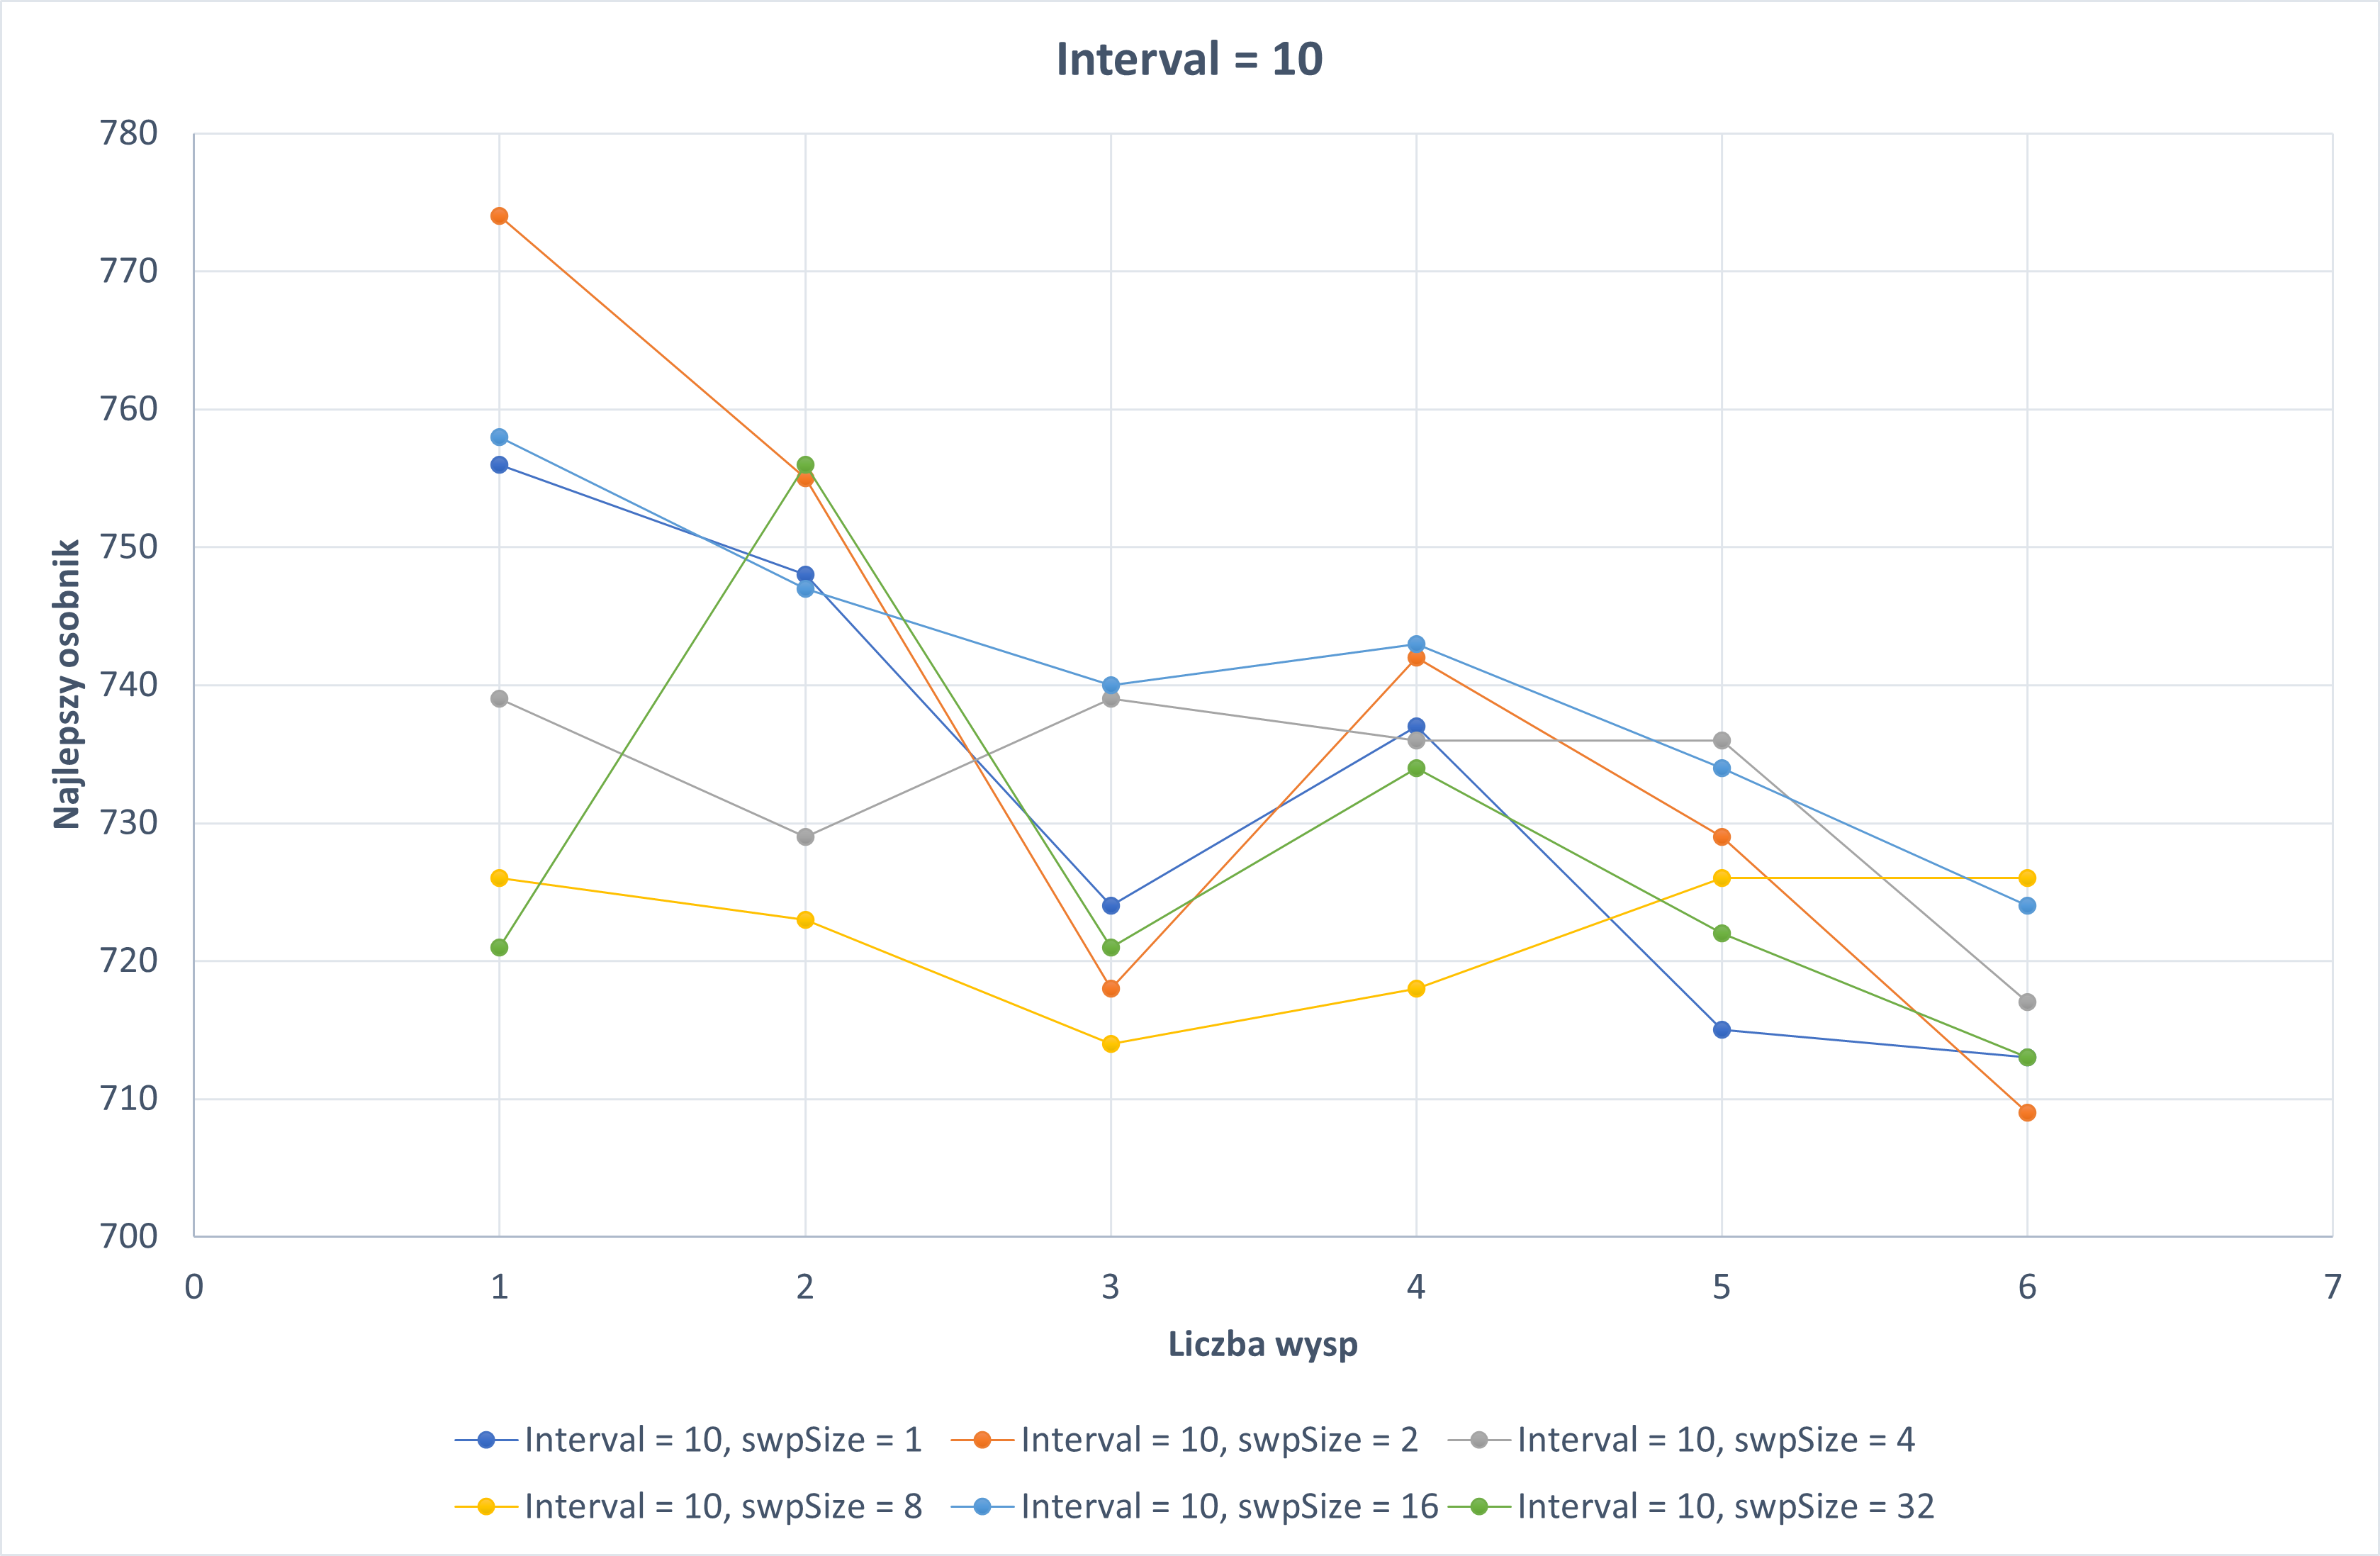
\includegraphics[scale=0.72]{Interval=10.png}
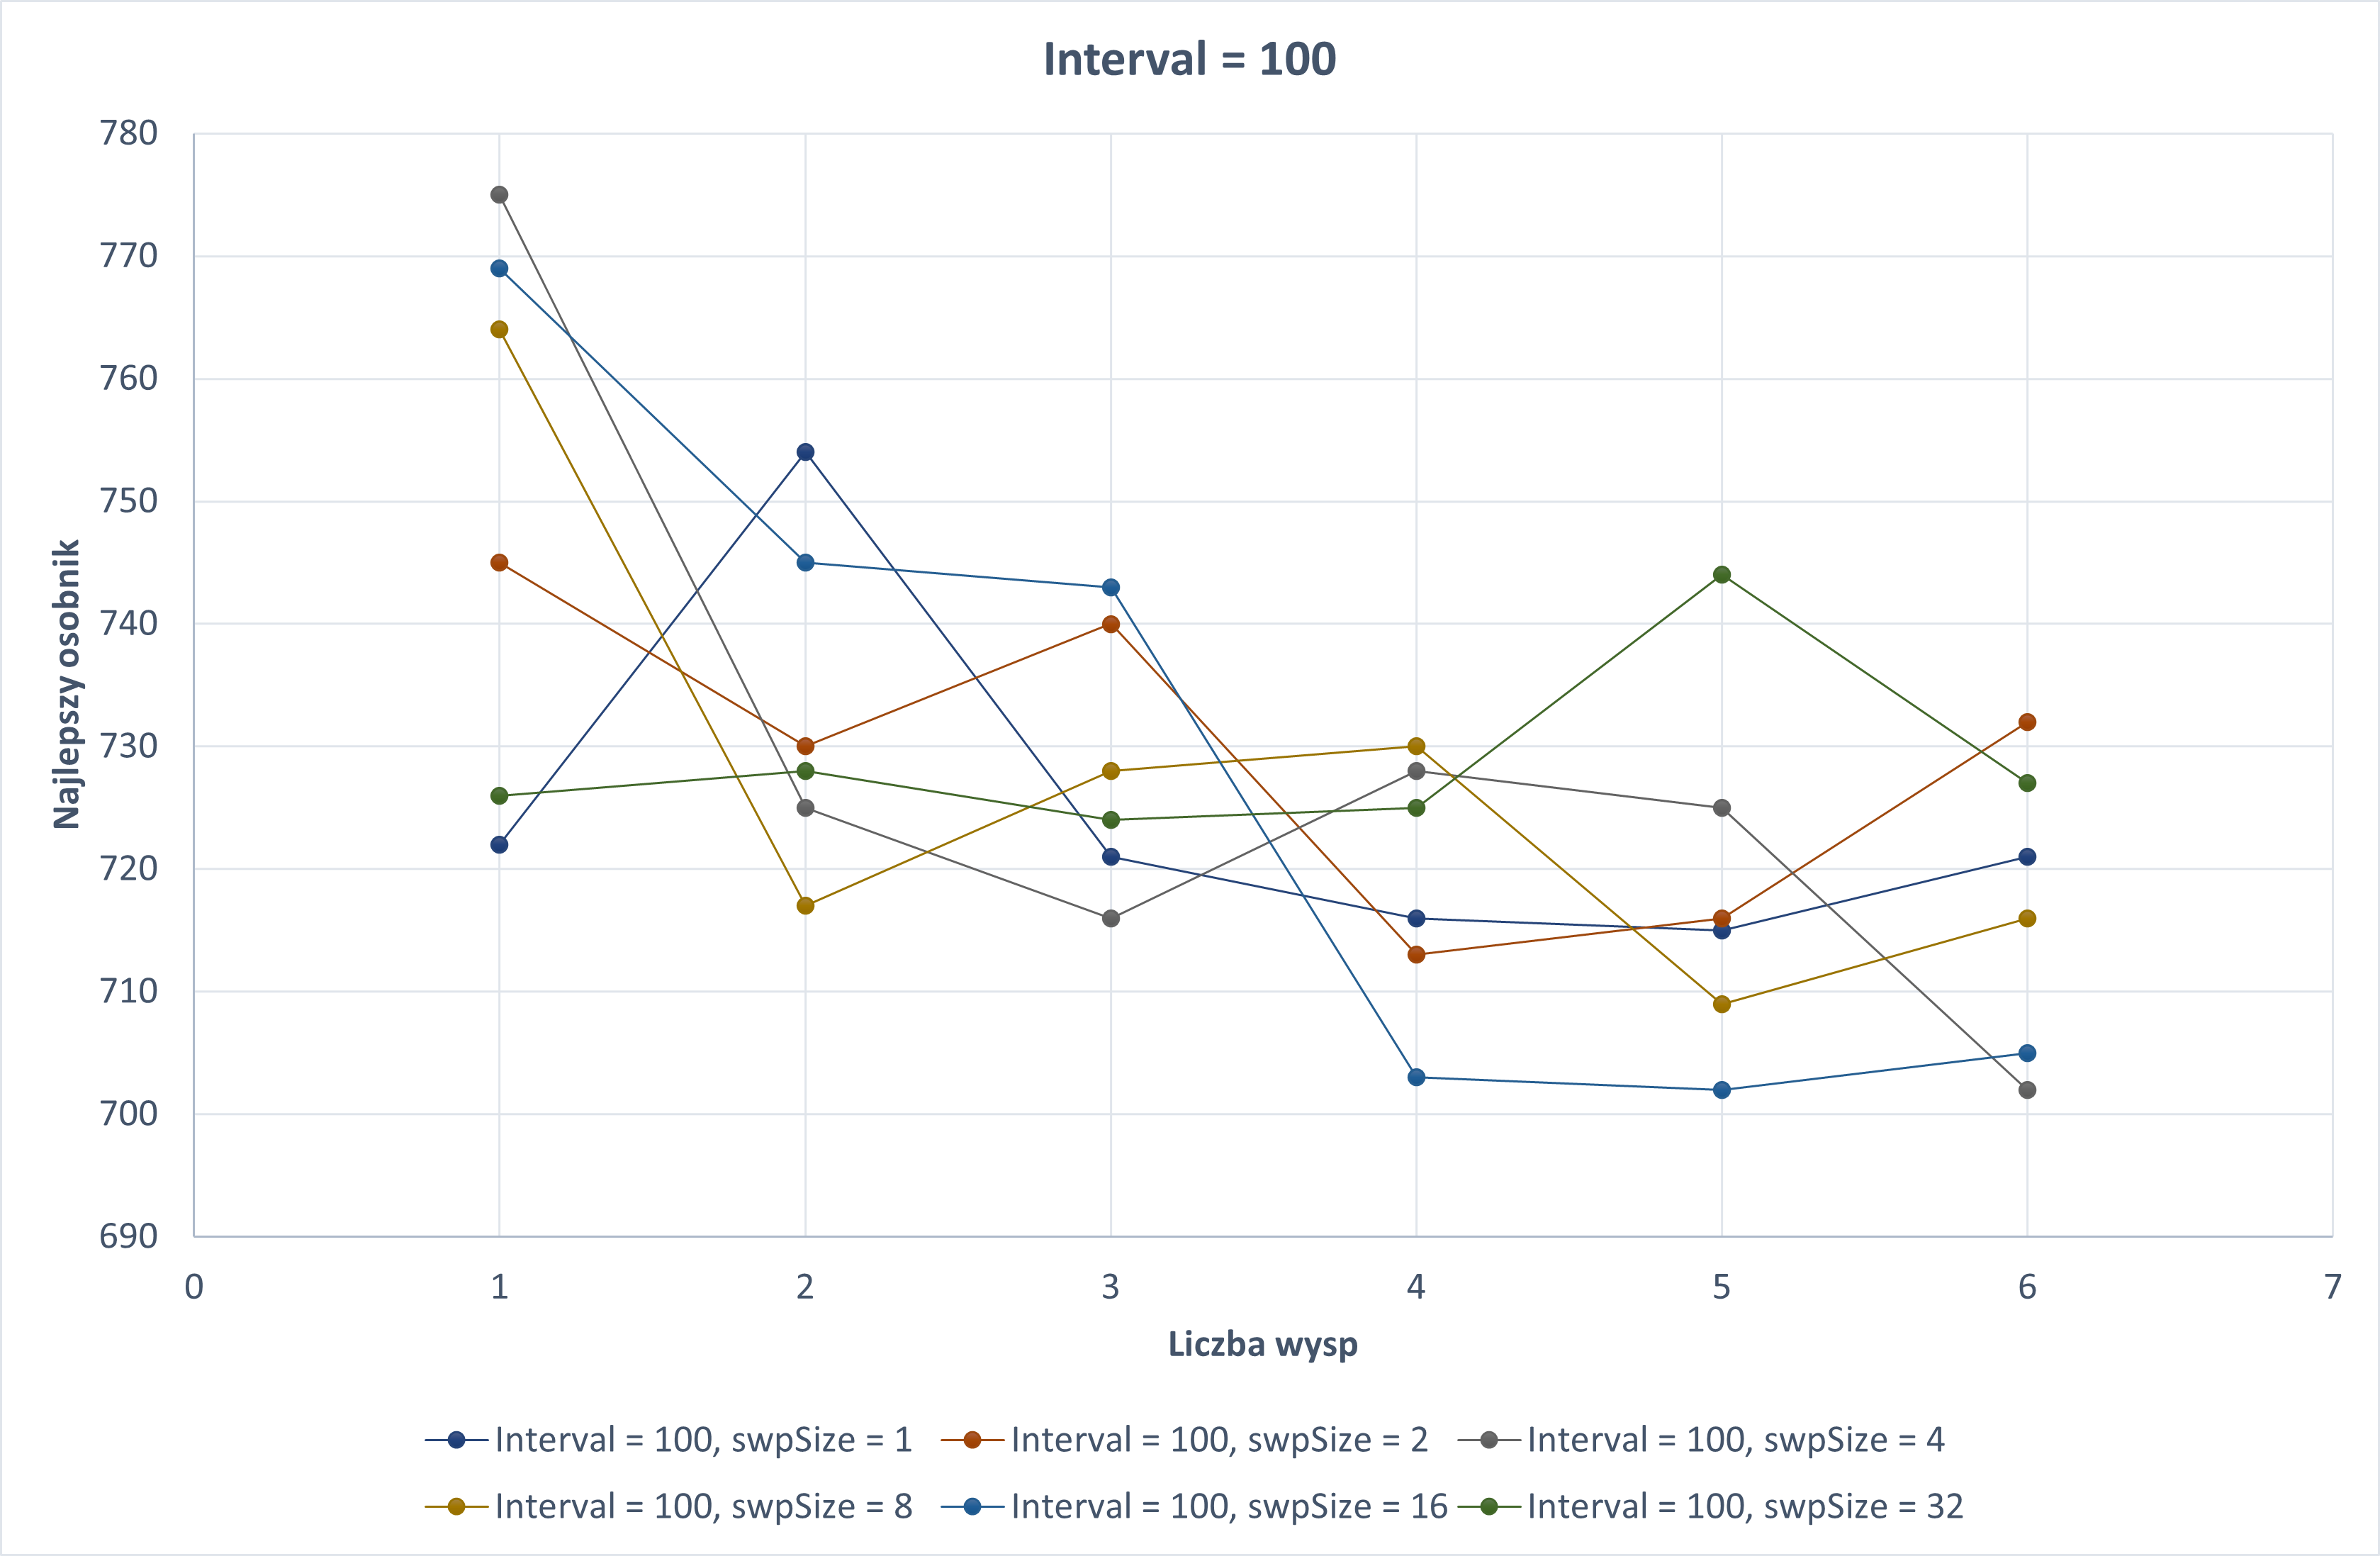
\includegraphics[scale=0.72]{Interval=100.png}
\includegraphics[scale=0.72]{Interval=1000.png}

\subsubsection*{Wpływ liczby osobników podlegających mieszaniu}
\includegraphics[width={\textwidth}/2]{swpSize=1.png}
\includegraphics[width={\textwidth}/2]{swpSize=2.png}
\includegraphics[width={\textwidth}/2]{swpSize=4.png}
\includegraphics[width={\textwidth}/2]{swpSize=8.png}
\includegraphics[width={\textwidth}/2]{swpSize=16.png}
\includegraphics[width={\textwidth}/2]{swpSize=32.png}

Na każdym z wykresów mniej lub bardziej, ale zawsze widać tendencję spadkową, co pozwala zakładać, że model wyspowy został zaimplementowany prawidłowo. Ulepszenie nie jest liniowe, ale skuteczne. Najszybszy zysk widać przy długich interwałach pomiędzy mieszaniem, w przypadku \texttt{Interval=1000} wartość funkcji celu już przy dwóch wyspach była znacznie lepsza od pojedyńczej, potem jednak zyski kolejnych wysp były mniejsze. Dla parametru liczby osobników branych do mieszania nie widać szczególnie jakiś własności, poza nieprzewidywalnością wyniku, kiedy bierzemy tylko po jednym z osobników.

\newpage
\section{Tabele Dodatkowe}

\begin{table}[h!]
	\centering
	\begin{tabular}{c||c|c|c|c|c||c|c}
Tabela D1.\\
Wspólne\\
Id & StartMode & SelectionMode & MutMode & CrossMode & CrossType & Sum & Avg \\
\hline
76 & 1 & 0 & 0 & 1 & 1 & 810.8125 & 50.67578125 \\
75 & 1 & 0 & 0 & 1 & 0 & 791.4375 & 49.46484375 \\
77 & 1 & 0 & 0 & 1 & 2 & 784.875 & 49.0546875 \\
115 & 1 & 1 & 0 & 2 & 1 & 876.875 & 54.8046875 \\
113 & 1 & 1 & 0 & 1 & 2 & 885.625 & 55.3515625 \\
112 & 1 & 1 & 0 & 1 & 1 & 923.5 & 57.71875 \\
114 & 1 & 1 & 0 & 2 & 0 & 931.125 & 58.1953125 \\
103 & 1 & 0 & 3 & 1 & 1 & 1129.1875 & 70.57421875 \\
116 & 1 & 1 & 0 & 2 & 2 & 1051.875 & 65.7421875 \\
111 & 1 & 1 & 0 & 1 & 0 & 1049.25 & 65.578125 \\
80 & 1 & 0 & 0 & 2 & 2 & 945.8125 & 59.11328125 \\
139 & 1 & 1 & 3 & 1 & 1 & 1139.875 & 71.2421875 \\
107 & 1 & 0 & 3 & 2 & 2 & 1210.125 & 75.6328125 \\
106 & 1 & 0 & 3 & 2 & 1 & 1291.25 & 80.703125 \\
142 & 1 & 1 & 3 & 2 & 1 & 1279.4375 & 79.96484375 \\
79 & 1 & 0 & 0 & 2 & 1 & 1093.1875 & 68.32421875 \\
143 & 1 & 1 & 3 & 2 & 2 & 1387.3125 & 86.70703125 \\
138 & 1 & 1 & 3 & 1 & 0 & 1344.8125 & 84.05078125 \\
141 & 1 & 1 & 3 & 2 & 0 & 1335.875 & 83.4921875 \\
149 & 2 & 0 & 0 & 1 & 2 & 1129.125 & 70.5703125 \\
104 & 1 & 0 & 3 & 1 & 2 & 1377.6875 & 86.10546875 \\
78 & 1 & 0 & 0 & 2 & 0 & 1200.875 & 75.0546875 \\
102 & 1 & 0 & 3 & 1 & 0 & 1441.9375 & 90.12109375 \\
140 & 1 & 1 & 3 & 1 & 2 & 1511.75 & 94.484375 \\
186 & 2 & 1 & 0 & 2 & 0 & 1361.6875 & 85.10546875 \\
210 & 2 & 1 & 3 & 1 & 0 & 1498.25 & 93.640625 \\
105 & 1 & 0 & 3 & 2 & 0 & 1359 & 84.9375 \\
152 & 2 & 0 & 0 & 2 & 2 & 1386 & 86.625 \\
148 & 2 & 0 & 0 & 1 & 1 & 1344 & 84 \\
187 & 2 & 1 & 0 & 2 & 1 & 1421 & 88.8125 \\
184 & 2 & 1 & 0 & 1 & 1 & 1365.125 & 85.3203125 \\
185 & 2 & 1 & 0 & 1 & 2 & 1404.5625 & 87.78515625 \\
178 & 2 & 0 & 3 & 2 & 1 & 1666.8125 & 104.17578125 \\
151 & 2 & 0 & 0 & 2 & 1 & 1436.0625 & 89.75390625 \\
150 & 2 & 0 & 0 & 2 & 0 & 1555.5625 & 97.22265625 \\
89 & 1 & 0 & 1 & 2 & 2 & 1605.0625 & 100.31640625 \\
213 & 2 & 1 & 3 & 2 & 0 & 1673.5 & 104.59375 \\
179 & 2 & 0 & 3 & 2 & 2 & 1722.5625 & 107.66015625 \\
183 & 2 & 1 & 0 & 1 & 0 & 1596.75 & 99.796875 \\
188 & 2 & 1 & 0 & 2 & 2 & 1606.75 & 100.421875 \\
88 & 1 & 0 & 1 & 2 & 1 & 1695.8125 & 105.98828125 \\
211 & 2 & 1 & 3 & 1 & 1 & 1879.125 & 117.4453125 \\
147 & 2 & 0 & 0 & 1 & 0 & 1718.4375 & 107.40234375 \\
81 & 1 & 0 & 1 & 0 & 0 & 1623.125 & 101.4453125 \\
175 & 2 & 0 & 3 & 1 & 1 & 1874.625 & 117.1640625 \\
125 & 1 & 1 & 1 & 2 & 2 & 1875.3125 & 117.20703125 \\
214 & 2 & 1 & 3 & 2 & 1 & 2064.4375 & 129.02734375 \\
72 & 1 & 0 & 0 & 0 & 0 & 1665.1875 & 104.07421875 \\
212 & 2 & 1 & 3 & 1 & 2 & 1916.25 & 119.765625 \\
123 & 1 & 1 & 1 & 2 & 0 & 1920.1875 & 120.01171875 \\

	\end{tabular}
\end{table}

\begin{table}[h!]
	\centering
	\begin{tabular}{c||c|c|c|c|c||c|c}
Tabela D2 (2 Pisemnie)\\
Id & StartMode & SelectionMode & MutMode & CrossMode & CrossType & Sum & Avg \\
\hline
107 & Hybryda & Turniej & Losowa & Part.Map. & Size/2 & 98 & 12.25 \\
102 & Hybryda & Turniej & Losowa & Mod.Ord.B. & All Par & 124 & 15.5 \\
106 & Hybryda & Turniej & Losowa & Part.Map. & Size/2 & 127 & 15.875 \\
103 & Hybryda & Turniej & Losowa & Mod.Ord.B. & Pop=20 & 141 & 17.625 \\
142 & Hybryda & Ruletka & Losowa & Part.Map. & Pop=20 & 161 & 20.125 \\
139 & Hybryda & Ruletka & Losowa & Mod.Ord.B. & Pop=20 & 163 & 20.375 \\
140 & Hybryda & Ruletka & Losowa & Mod.Ord.B. & Size/2 & 188 & 23.5 \\
143 & Hybryda & Ruletka & Losowa & Part.Map. & Size/2 & 197 & 24.625 \\
138 & Hybryda & Ruletka & Losowa & Mod.Ord.B. & All Par & 202 & 25.25 \\
104 & Hybryda & Turniej & Losowa & Mod.Ord.B. & Size/2 & 206 & 25.75 \\
	\end{tabular}
\end{table}
\end{document}